%\documentclass[10pt]{article}
\documentclass[10pt]{book}

\usepackage[draft]{fixme}

\usepackage{listings}

\usepackage{html}
\usepackage{color}

\usepackage{multicol}
\usepackage{multirow}

\usepackage{graphicx}
\usepackage{alltt}

\newcommand{\hlstd}[1]{\textcolor[rgb]{0,0,0}{#1}}
\newcommand{\hlkey}[1]{\textcolor[rgb]{0,0,0}{\bf{#1}}}
\newcommand{\hlnum}[1]{\textcolor[rgb]{0.16,0.16,1}{#1}}
\newcommand{\hltyp}[1]{\textcolor[rgb]{0.51,0,0}{#1}}
\newcommand{\hlesc}[1]{\textcolor[rgb]{1,0,1}{#1}}
\newcommand{\hlstr}[1]{\textcolor[rgb]{1,0,0}{#1}}
\newcommand{\hldstr}[1]{\textcolor[rgb]{0.51,0.51,0}{#1}}
\newcommand{\hlcom}[1]{\textcolor[rgb]{0.51,0.51,0.51}{\it{#1}}}
\newcommand{\hldir}[1]{\textcolor[rgb]{0,0.51,0}{#1}}
\newcommand{\hlsym}[1]{\textcolor[rgb]{0,0,0}{#1}}
\newcommand{\hlline}[1]{\textcolor[rgb]{0.33,0.33,0.33}{#1}}

\newcommand{\mySmallFontSize}{\scriptsize}
\newcommand{\mySmallestFontSize}{\tiny}

\newcommand{\codeFontSize}{\scriptsize}
\newcommand{\code}[1]{{\scriptsize #1}}

% Software version number
\newcommand{\VersionNumber}{0.11.13.0}

\newcommand{\ExampleDirectory}{/home/meltdown1995/roseRoot/rose-compiler//src/projects/compass/tests}

% Latex trick to allow us to comment out large sections of documentation
\newcommand{\commentout}[1]{}

% change the title of the Fixme List
\renewcommand{\listfixmename}{Things to Fix in Documentation of Compass}

\newcommand{\comm}[2]{\bigskip
                      \begin{tabular}{|p{11cm}|}\hline
                      \multicolumn{1}{|c|}{{\bf Comment by #1}}\\ \hline
                      #2\\ \hline
                      \end{tabular}
                      \bigskip
                     }

\def\verbatimfile#1{\begingroup
                    \@verbatim \frenchspacing \@vobeyspaces
                    \input#1 \endgroup
}



\newcounter{lineno}

% Taken from verbatimfiles.sty on web
\makeatletter %JCL

\def\verbatimlisting#1{\setcounter{lineno}{0}%
    \begingroup \@verbatim \frenchspacing \@vobeyspaces \parindent=20pt
    \everypar{\stepcounter{lineno}\llap{\thelineno\ \ }}\input#1
    \endgroup
}

\makeatother %JCL

% \endinput


%\addtolength{\oddsidemargin}{-0.5in}
%\addtolength{\evensidemargin}{-0.5in}
\addtolength{\textheight}{0.5in}
%\addtolength{\textwidth}{0.5in}
%\addtolength{\textwidth}{1.0in}
%\addtolength{\topmargin}{-0.5in}
%\addtolength{\textheight}{1.5in}

% \pagenumbering{roman}
% \pagestyle{empty}
% \setcounter{page}{0}
% \thispagestyle{empty}

\sloppy

%---------------------------------------------------------------------
% Begin Document
%---------------------------------------------------------------------

\begin{document}
%\bibliographystyle{plain}
%

% This draft mode eliminates the figures (leaves boxes for where they would be)
%\psdraft

\title{ {\bf \textcolor{red}{         Compass User Manual: \\ 
                                A Tool for Source Code Checking \\
                                        (A ROSE Tool)} \\
                               \textcolor{blue}{Draft User Manual} \\
                               \textcolor{green}{(Associated with ROSE Version 0.11.13.0)} } }

\author{ {\bf ROSE Team} \\
         Lawrence Livermore National Laboratory \\ 
         Livermore, CA  94550 \\
         925-423-2668 (office)  925-422-6278 (fax) \\
         {dquinlan}@llnl.gov \\
         Project Web Page: http://www.rosecompiler.org \\
         %Project Web Page: www.llnl.gov/casc/rose \\
         UCRL Number for ROSE User Manual: UCRL-SM-210137-DRAFT \\
         UCRL Number for ROSE Tutorial: UCRL-SM-210032-DRAFT \\
         UCRL Number for ROSE Source Code: UCRL-CODE-155962 \\ \\
         %\htmladdnormallink{ROSE User Manual (pdf)}{../ROSE_UserManual/ROSE-0.11.13.0-UserManual.pdf} \\
         \htmladdnormallink{ROSE User Manual
         (pdf)}{http://www.rosecompiler.org/ROSE_UserManual/ROSE-0.11.13.0-UserManual.pdf} \\
         \htmladdnormallink{ROSE Tutorial
         (pdf)}{http://www.rosecompiler.org/ROSE_Tutorial/ROSE-0.11.13.0-Tutorial.pdf} \\
         \htmladdnormallink{ROSE HTML Reference (html
         only)}{http://www.rosecompiler.org/ROSE_HTML_Reference/index.html}
       }

% \textcolor{blue}{Compiler infrastructure for tools is a bit} \\
% \textcolor{blue}{like a cannon, sometime more than you really need,} \\ 
% \textcolor{blue}{but often all that it takes to solve the problem} \\

% This doesn't seem to work.  References to this label are not resolved.
\label{Compass:postscriptVersionOfUserManual}

\begin{htmlonly}
   \centering \includegraphics[width=3in]{../compass_rose.gif}
\end{htmlonly}

\maketitle

\begin{htmlonly}
   \centering \includegraphics[width=5in]{../compass_rose.gif}
\end{htmlonly}


%\begin{center}
%\today
%\end{center}

%\newpage
%\input{Copyright}
%\newpage

\newpage

%
\chapter*{Preface}

%  Purpose:
% \begin{itemize}
%    \item a. Welcome 
%    \item b. Program features
%    \item c. Program benefits
% \end{itemize}
% \begin{center}
% *********************  \newline
% \end{center}
% \vspace{0.25in}

   Welcome to the ROSE Compiler Framework Project.  The purpose of this project is to 
provide a mechanism for construction of specialized source-to-source translators 
(sometime referred to less precisely as {\em preprocessors}).  ROSE provides 
simple programmable mechanisms to read and rewrite the abstract syntax trees generated 
by separate compiler front-ends.  ROSE includes the Edison Design Group (EDG) 
front-end (in binary form within public
distributions), and is internally based upon SAGE III, thus ROSE is presently specific 
to the generation of C and C++ source-to-source based compilers ({\em translators}, 
more precisely).  Other language front-ends may be appropriate to add to ROSE in 
the future (current work with Rice University is focused on the addition of Open64's
front-end to ROSE as part of support for FORTRAN 90).

   ROSE makes it easy to build complex source-to-source translator
(preprocessor) tools, and thus supports research work in many areas:
\begin{itemize}
   \item Performance Optimization
   \item General Program Transformations
   \item Instrumentation
   \item Program Analysis
   \item Interface Generation
   \item Automated Check-pointing
   \item Software Security Analysis
   \item Software Verification
   \item Automated Unit Test Generation
   \item ... and much more ...
\end{itemize}


%\input{Forward}

% This fixes the really long table of contents problem
\setcounter{tocdepth}{1}

\tableofcontents
%\listoffigures
%\listoftables
\newpage
%


% \chapter*{Acknowledgments}
\chapter*{Acknowledgments}

% \begin{center}
% ********  To be removed later  *************  \newline
% \end{center}
% 
%  Purpose:
% \begin{itemize}
%    \item A. Thank everyone
% \end{itemize}
% \begin{center}
% *********************  \newline
% \end{center}
% \vspace{0.25in}
% 

   The Intermediate Representation (IR) used in ROSE is called SAGE III.
SAGE III is something that we have built based on SAGE II, which was never 
completed or widely distributed. SAGE II was based on SAGE++, the improvements 
over SAGE++ were significant. SAGE II was the first version of SAGE to use the 
Edison Design Group (EDG) frontend.  We want to thank the original
developers of SAGE++ and SAGE II for their work, from which we learned a lot
through use of their object-oriented IR interface.

   We chose the name SAGE III to give sufficient credit to the original developers
of SAGE++ and SAGE II, who also suggested that we call what we are doing SAGE III.  
ROSE, of course, builds on SAGE III and adds numerous additional mechanisms, 
including:
\begin{itemize}
    \item Loop Optimizations (called by ROSE users)
    \item Abstract Syntax Tree (AST) Attributes (tree decoration)
    \item A family of AST Traversals (as used with Attribute Grammars)
    \item AST Rewrite mechanisms
    \item AST Query Mechanisms
    \item C and C++ code generation from SAGE III
    \item AST File I\/O
    \item Significant robustness for C, C99, and C++ (handles large DOE applications)
    \item AST Visualization
    \item and more ...
\end{itemize}

   SAGE III is an automatically generated body of software that uses ROSETTA, a tool we 
wrote and distribute with ROSE. ROSETTA is an IR generator that, as its largest and most
sophisticated test, generates SAGE III.  The connection code that was used to translate 
EDG's AST to SAGE II was derived loosely from the EDG C++ source generator and has
formed the basis of the SAGE III translator from EDG to SAGE III's IR. Under this license
we exclude the EDG source code and the translation from the EDG AST in distributions 
and make available only a binary of those parts with use EDG (front-end AST translation),
and the source to all of ROSE (which does not depend on EDG). No part of the EDG work is 
visible to the user of ROSE.  We can make the EDG source available only to those who have 
the free EDG research license.  We want to thank the developers at Edison Design Group
(EDG) for making their work so widely available under their research license program.

   Markus Schordan was the first post-doctorate researcher on the ROSE project; he made 
significant contributions while employed at Lawrence Livermore National Laboratory (LLNL), 
including the AST traversal mechanism.  We continue to work with Markus, who is now at 
Vienna University of Technology as an Associate Professor. We were also fortunate to 
leverage a significant portion of Qing Yi's thesis work (under Ken Kennedy) 
% on loop optimizations as part of her post-doc at Lawrence Livermore National Laboratory with the ROSE project, 
and we would like to thank her for that work and the work she did as a post-doc at Lawrence Livermore National Laboratory. 
We continue to work with her, although she is now at the University of Texas at San Antonio.

     There are many additional people to thank for our current status in 
% where we are currently within 
the ROSE project:
\begin{itemize}
     \item Contributing Collaborators: \\
           Markus Schordan (Vienna University of Technology),
           Rich Vuduc (Georgia Tech), and
           Qing Yi (University of Texas at San Antonio)

     \item Post-docs (including former post-docs): \\
           Chunhua Liao (from University of Houston),
           Thomas Panas (from Vaxjo University, Sweden),
           Markus Schordan (from University of Klagenfurt, Austria),
           Rich Vuduc (from University of California at Berkeley), and
           Jeremiah Willcock (from Indiana University),
           Qing Yi (from Rice University)
     \item Students: \\
           Gergo Barany (Technical University of Vienna),
           Michael Byrd (University of California at Davis),
           Gabriel Coutinho (Imperial College London),
           Peter Collingbourne (Imperial College London),
           Valentin David (University of Bergen, Norway),
           Jochen Haerdtlein (University of Erlanger, Germany),
           Vera Hauge (University of Oslo, Norway),
           Christian Iwainsky (University of Erlanger, Germany),
           Lingxiao Jiang (University of California at Davis),
           Alin Jula (Texas A\&M),
           Han Kim (University of California at San Diego),
           Milind Kulkarni (Cornell University),
           Markus Kowarschik (University of Erlanger, Germany),
           Gary Lee (University of California at Berkeley and Purdue University),
           Chunhua Liao (University of Houston),
           Ghassan Misherghi. (University of California at Davis),
           Peter Pirkelbauer (Texas A\&M),
           Bobby Philip (University of Colorado),
           Radu Popovici (Cornell University),
           Robert Preissl (xxx Austria),
           Andreas Saebjornsen (University of Oslo, Norway),
           Sunjeev Sikand (University of California at San Diego),
           Andy Stone (Colorado State University at Fort Collins),
           Ryan Stutsman (Stanford University),
           Danny Thorne (University of Kentucky), 
           Nils Thuerey (University of Erlanger, Germany), 
           Ramakrishna Upadrasta (Colorado State University at Fort Collins),
           Christian Wiess(Munich University of Technology, Germany), 
           Jeremiah Willcock (Indiana University),
           Brian White (Cornell University),
           Gary Yuan (University of California at Davis), and
           Yuan Zhao (Rice University).
     \item Friendly Users: \\
           Paul Hovland (Argonne National Laboratory),
           Brian McCandless (Lawrence Livermore National Laboratory),
           Brian Miller (Lawrence Livermore National Laboratory),
           Boyana Norris (Argonne National Laboratory),
           Jacob Sorensen (University of California at San Diego),
           Michelle Strout (Colorado State University),
           Bronis de Supinski (Lawrence Livermore National Laboratory),
           Chadd Williams (University of Maryland),
           Beata Winnicka (Argonne National Laboratory),
           Ramakrisna xxx (Colorado State University at Fort Collins), and
           Andy Yoo (Lawrence Livermore National Laboratory)
     \item Support: \\
           Steve Ashby,
           David Brown,
           Bill Henshaw,
           Bronis de Supinski, and
           CASC management
     \item Funding: \\
           Fred Johnson (Department of Energy, DOE) and
           Mary Zosel (Lawrence Livermore National Laboratory)
\end{itemize}

\fixme{Check spelling of student names.}

To be clear, nobody is to blame for the poor state of the current version of the 
ROSE documentation (but myself).

% At some point we should add Michelle
% Michelle Strout (Colorado State University)
% and perhaps Jacob
% Jacob Sorenson (UCSD),

% including Kei, Fede, Bobby, Bill, and David. And nobody to blame for the 
% poor state of the current version of the ROSE documentation (but myself).





\newpage

\chapter{Introduction}

\quote{A software analysis story about four people named: Everybody, Somebody, Anybody, and Nobody.
There was an important job to be done and Everybody was sure that Somebody would do it.
Anybody could have done it, but Nobody did it.  Somebody got angry about that because
it was Everybody's job.  Everybody thought that Anybody could do it, but Nobody
realized that Everybody wouldn't do it. It ended up that Everybody blamed Somebody
when Nobody did what Anybody could have done.}
\footnote{Story not really specific to softare analysis found at
 http://www.corsinet.com/braincandy/hlife.html}


\section{Overview}

\label{introduction::overview}

   Compass is a tool for the checking of source code.  It is
based on the ROSE compiler infrastructure and demonstrates to
use of ROSE to build lots of simple pattern detectors for analysis
of C, C++, and Fortran source code.

   The purpose of this work is several fold:
\begin{itemize}
   \item Provide a concrete tool to support interactions with lab customers.
   \item Provide a home for the security analysis specific detectors being built within
         external research projects.
   \item Provide an external tool for general analysis of software.
   \item Provide a tool to support improvements to the ROSE source code base.
   \item Define an infrastructure for an evolving and easily tailored program analysis tool.
   \item Provide a simple motivation for expanded use of ROSE by external users.
         Development, testing, and evaluation of ROSE infrastructure is best facilitated 
         through its expanded use by others and this provides a specific and attractive
         tool that can provide feedback to users about their own code projects.  Even
         though optimization research is our focus, this gets our supporting
         infrastructure for optimization research out and into use by others in the form
         of an extensible tool.
\end{itemize}

   Note that as the collection of detectors grows we will periodically reorganize the 
collection.  At some point soon we will build a hierarchy to organize the evolving
collection.

%\subsection{A basis for other source analysis tools}
\paragraph{A basis for other source analysis tools}
   Input and output to ROSE is organized so that any number of sources could be used.
So although we provide a compiler interface (for simplicity), we will also provide a 
GUI interface as an alternative interface to demonstrate that the detectors are orthogonal
to there use in alternative tools.  Alternative tool interfaces should be possible 
and will further demonstrate the independence of the input and output mechanisms to
the designs and implementation of the core detectors.

\paragraph{Add Your Own Detector}

    Detectors written in Compass make direct use of ROSE and are 
designed to be copied and extended by users to develop their own 
detectors. We welcome the contribution of these detectors back to 
the ROSE team for inclusion into future releases of Compass;
full credit for all work will be provide to all authors.
Compass is an open source project using ROSE, an open source
compiler infrastructure.

    Each of the detectors are examples of how to
add your own detector to {\bf Compass}.  If you
build a detector that you would like to have be 
distributed with {\bf Compass}, please send it to
us and we will add your as an external contributor.

  Guidelines for contributions:
\begin{itemize}
   \item Use any Compass detector and an example.
   \item provide the documentation about your detector.
   \item Use any features in ROSE to support your detector; AST, Control Flow graph,
    System dependence Graph, Call Graph, Class Hierarchy Graph, etc.
   \item Your detector should have {\bf NO} side-effects on the AST.
\end{itemize}







\newpage


\chapter{Design and Verification}

Compass is a tool is used to analyze software (both source code and binaries). 
A collection of {\em checkers} are built with each of them detecting the 
violation of a rule.  By reporting on the violations of rules {\em Compass} provides 
a way to enforce predefined or arbitrary user specified properties on software.
This chapter covers the design of {\em Compass} and the design of the verification in 
the \emph{Compass Verifier}, used to verify properties of the checkers implemented 
and submitted to {\em Compass}.

% \section{Use Cases}
\section{Usage Model}

\label{design::UseCase}

Figure~\ref{Compass_usecase} shows the usage model (use cases) of \emph{Compass}.
The analysis is triggered by the user running {\em Compass} over an
input file (source code or binary). The user implicitly selects 
which checkers to execute (defining what rules are to be enforced); 
by default all checkers are run. 
The user also specifies the input file to be checked; for source code 
the specification is similar to the command line required for the 
compilation in the case of a source file.  Results of the analysis 
are presented to the user, a number of mechanisms can be used to 
display the results.

\begin{figure}[th]
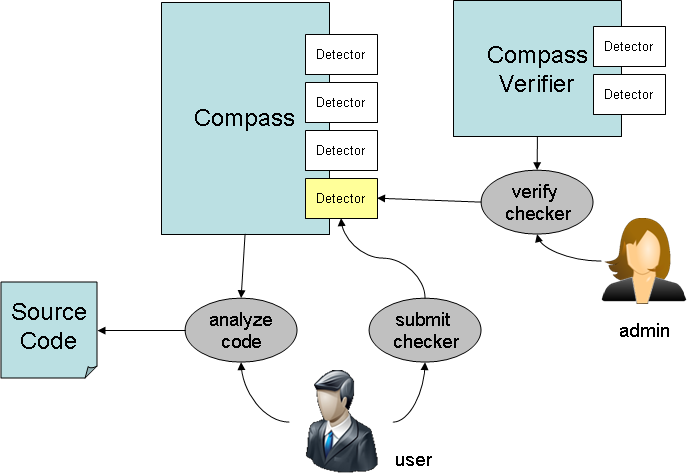
\includegraphics[width=4.5in]{compass_pic.png}
\caption{Compass Use Case}
\label{Compass_usecase}
\end{figure}

Either the same user or a different user/developer can also
implement and submit checkers to be built into Compass.
% Furthermore, a user may contribute with his own checkers that can be added to Compass. 
Since external users may contribute checker automatically via scripts, a verification of the 
validity and safety of these checkers is necessary. We provide a \emph{Compass Verifier}
that helps to check that all checkers are safe. Currently, the verifier is run by
an administrative person but may run automatically in the future.

%\section{Assumption of trust} 
\section{Trust Model}
By design we make a few assumptions about the use of Compass in order to define
a secure tool. We assume:
\begin{enumerate}
   \item For now, there is an assumption of trust in the person writing the checker. \\
      We use the \emph{Compass Verifier} as a way to double check the 
      checkers so that we can eventually weaken the level of trust assumed for people 
      writing checkers. However, the design of the \emph{Compass Verifier} is not likely to
      ever be robust enough to guarantee an automated proof of security for each checker.  
      Thus, we also assume that someone trusted will also review the checker.
      {\em not implemented: We expect that a digital signature (using a key mechanism) 
           is possible to associate a trusted reviewer with a review of 
           the checker together with a strong hash function that
           digitally signs the checker source code.}

   \item Since running \emph{Compass Verifier} is an optional part of building 
      the Compass executable, the person running these test is trusted. There are
      two ways to run the \emph{Compass Verifier} (see section \ref{sec:compass_verify}
    for details):
      \begin{itemize}
         \item Slow: once on each checker ({\tt make verify}). This mechanism
            tests all the files one checker at a time and thus can not miss 
            a file.  Note that even the counter examples are tests which can 
            be a problem when the counter example for the checker is detected
            as a violation for \emph{Compass Verifier}.  Counter examples for
            checkers have to be carefully written to not represent examples that
            violate \emph{Compass Verifier}.
         \item Fast: once on the union of all the checkers ({\tt make oneBigVerify}).
            This step forms a single file of all the checkers (and in-doing so can
            miss some files, and so is less secure).  It is mostly for testing 
            purposes.
      \end{itemize}

   \item The person building the Compass executable is trusted.

   \item The environment where the testing using Compass is done is trusted.

   \item Compass is designed so that the user running Compass need not be trusted.

\end{enumerate}

It is unclear at present how weak the assumption of trust on the compass checker developer 
can be and it may ultimately depend directly on the capabilities of the \emph{Compass Verifier}.


\section{Architecture}

\begin{figure}[thb]
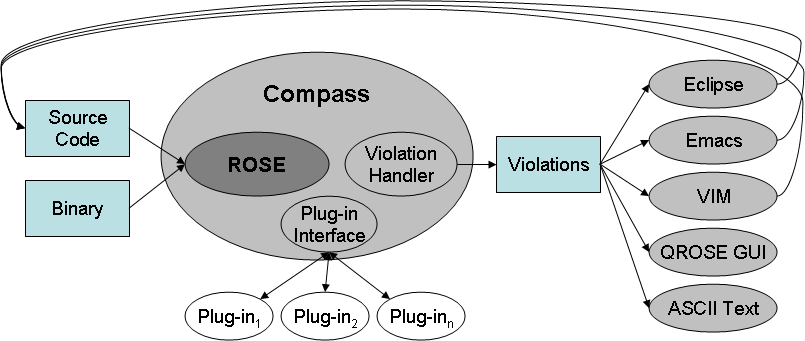
\includegraphics[width=6.0in]{compass_arc.png}
\caption{Compass Architecture}
\label{CompassArchitecture}
\end{figure}


Compass is a tool that allows users to implement checkers to locate and
report software defects.
Documentation of various kinds of software defects can be found in sources
such as the CERT Secure Coding Rules, Common Weakness Enumeration from MITRE, 
and other sources. Our focus is not to define new software defects but
rather to provide a platform that allows the easy implementation of defect
checkers.  Compass has been designed to be easy to extend, allowing users to 
implement their own custom checkers (custom source code analyses for
identifying defects), as shown in Figure~\ref{CompassArchitecture}. Compass supports
the implementation of both simple as well as more advanced defect
checkers. For the latter, Compass utilizes the ROSE infrastructure to
perform a wide range of general purpose program analyses, such as control
flow analysis, data flow analysis, program slicing, etc.


Compass is designed in a way that allows users who do not necessarily have
compiler backgrounds to utilize the ROSE infrastructure to build their
own analysis tools.
Compass is foremost an extensible open source infrastructure for the
development of large
collections of rules. Our current implementation supports automatic
defect checking, programming language restriction, and malware detection in
C, C++, and object code.
Support for Fortran is a new addition to ROSE and will be supported in
Compass in the near future.




\section{Design}

\begin{figure}[thb]
\hspace{-1.5in}
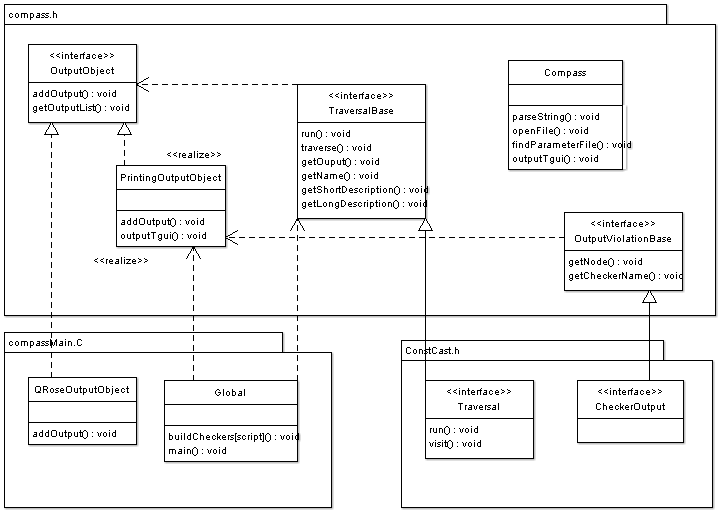
\includegraphics[width=7in]{compassdesign.png}
%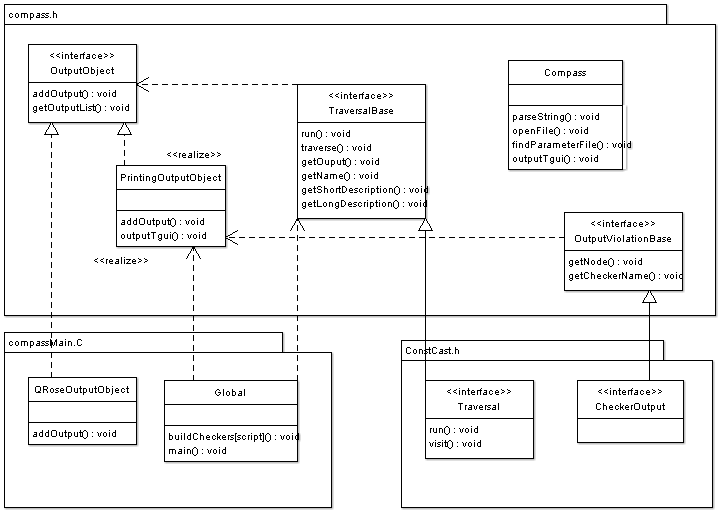
\includegraphics[width=6.0in]{compassdesign.png}
\caption{Compass Design}
\label{CompassDesign}
\end{figure}

Compass is designed to be easy to extend. Any user may write a checker and add it to
Compass. Figure~\ref{CompassDesign} illustrates the UML design decisions behind Compass.


Most of the functionality of Compass is in abstract classes hidden in the Compass
namespace within compass.h - a file within the compassSupport directory. The figure uses a
specific example, {\em ConstCast}, for illustration; Compass is designed to support a large
number of checkers (hundreds). All checkers, such as the {\em ConstCast} checker (illustrated in
figure~\ref{CompassDesign}), utilize the abstract classes to traverse a program with all
its nodes and to output violations found in that code according to the local algorithm.

CompassMain is the main executable that initially calls ROSE to parse a program. Then
\emph{buildCheckers} is called to load all checkers that are specified within a
configuration file. The configuration file allows users to turn on and turn off specific
checkers for their run-time analyses. However, the configuration file only permits
checkers to be loaded that were part of Compass at compile-time.

The main interface file compass.h contains the class \emph{Checker} and the
abstract class \emph{OutputObject}. Checker is the interface to ROSE,
giving the metadata for a checker and a function to apply the checker to a
given AST.
OutputObject aids
to output defects found by a specific checker. More functionality to handle e.g. file
input and parameters provided to Compass, is provided within the Compass namespace.

\section{Compass Verifier}

Compass must be safe, so that analyses and their results can be trusted. 
The {\em Compass Verifier} is used at build time to run a specific set of separate 
compass rules offer the source code of all the checkers.  For simplicity it runs in two
modes: fast, for checking specific named checker source files; and slow, for testing 
{\em all} checker source files.

\subsection{Threats} 

In order to define a complete design for security we outline the threats that
understand to be relevant. The main threats to the validity of Compass checkers are:
\begin{itemize}
\item \emph{Malicious User} \\ 
  A malicious user is an external user of Compass contributing a checker that performs malicious behavior.
\item \emph{Malicious Checker} \\ 
  Compass is extensible and new checkers can be added externally (users outside the main development group).
  A checker can be programmed arbitrarily using the C/C++ and assembly programming languages. 
  It is therefore possible for a skilled programmer to hide malicious operations within a
  checker.  Compass must prevent checkers with malicious behavior to be part of the
  Compass system. Threats are:
   \begin{itemize}
      \item {\bf exfiltration} \\
         A checker should act in a secure way with the input files it is given.
         Securing the inputs to Compass (e.g. the inputs to each checker) from 
         exfiltation is a first priority. Allowing a checker to scan the host 
         machine to exfiltrate arbitrary data (this is a threat that any secure
         software will have).
      \item {\bf modification of filesystem} \\
         A checker should be side-effect free, or have only well defined side-effects, 
         but a malicious checker could modify or erase parts of the accessible file 
         system (e.g. deleting whole directory structures).
%     \item {\bf others ??? ...}
   \end{itemize}

\item \emph{Malicious Compass} \\
    Since Compass is built from ROSE, it is possible to modify compass (or any checker) 
    to generate source code that could be compiled to replace the existing executable
    (there are some constraints here) or regenerate the source code to replace the 
    existing source code or perhaps just provide an alternative copy of the source code.
    This indirect transformation of the input code is a threat.

\item \emph{Source Code Replacement} \\ It should not be possible for users to exchange the
    source code of checkers within a running system, i.e. Compass cannot implement dynamic
    loading of checkers. Such a feature would compromise its safety.

\item \emph{Binary Replacement} \\ Another threat is the replacement of a valid Compass
    checker with a modified malicious version within a binary release of Compass.
    Therefore, Compass should be aware if parts of itself were modified and should not
    execute.

\end{itemize} 

%\subsection{Safety Handling}
\subsection{Mitigation of Threats}

Compass is designed to be safe. The Compass Verifier is a stable separate copy of Compass
that contains only a few checkers to check (external and internal) user delivered checkers
for safety.  We have hopefully designed Compass in a way that it addresses the threats
mentioned above:
\begin{itemize}
\item \emph{Malicious User} \\ Initially, we permit only trusted individuals to add new
    checkers to Compass. Once the verification process is matured, we will extend this
    policy to allow less trusted users to contribute to Compass. A goal will be to allow
    arbitrary users to contribute checkers, however, a review of the whole Compass design
    (and the {\em Compass Verifier} especially) will be required to define required trust
    levels for user/developers who implement checkers.
\fixme{We might define trusted and untrusted checkers as a way to have checkers from
       arbitrary users, but mark them as untrusted.}

\item \emph{Malicious Checker} \\ To prevent Compass from executing malicious code, the Compass
    Verifier executes its own checkers on any user defined checker that is being
    considered to be added to Compass. Currently, the Compass Verifier contains three checkers:
   \begin{itemize}
      \item \emph{fileReadOnlyAccess} ensures that a user defined checker performs no write
         or execute operations on files.
      \item \emph{allowedFunctions} is a {\em white list} of function calls permitted in
         a checker. This list contains functions that are trusted and hence considered
         safe when integrated to Compass.
\fixme{This is not yet implemented as a white list and is instead currently a black list; called: forbiddenFunctions.}
      \item \emph{noAsmStmtsOps} searches for assembly instructions in a checker and flags
         and reports all cases as unsafe.
      \item To avoid modifications of the AST for the purpose of allowing other checkers
         to pass, the AST should not be modified (this should extend to all the
         program analysis graphs generated and used by other checkers).
         {\em This is not implemented yet.} 
\end{itemize}

\item \emph{Malicious Compass} \\
    Since Compass does not generate code, it can not be used to modify the input software
    (source code or binary) or generate a new copy that could be confused with the input.
    However, future versions of Compass make make transformation to introduce greater
    levels of security; fix flaws, mitigate specific forms of threats, etc.  It will be
    important to make sure that such transformation can not change the behavior of an
    input code to make the modified input code malicious.  Current proposed approaches
    would build a patch which would have to be inspected by a trusted developer before
    it would be applied to modify the input code.

\item \emph{Source Code Replacement} \\ Checkers can only be added at compile time to
    Compass, not at run-time. This means that checkers (meaning the source code) cannot be
    exchanged against unsafe versions at run-time. Furthermore, we allow only the Compass
    tool builder (admin) to build versions of Compass that must pass the Compass Verifier.

\item \emph{Binary Replacement} \\ 
    Our goal is to perform a strong hash (e.g. Secure Hash Algorithm - SHA2) as a 
    checksum on all the checkers
    part of the binary Compass distribution before Compass is executed. In this way
    Compass will not run if parts of it were modified. {\em This is not implemented yet.}
\fixme{We should describe the policy for allowing SHA2 to be verified. Where the SHA2
    results for checkers would be published (e.g. web site), etc.}

\end{itemize} 


%The above list contains an important subset of checkers that enforce Compass checkers to be safe. 
%Additional checkers can easily be added to that list.
%In the future, a checker submitted to Compass, should go first through the automatic verifier, before it is either 
%added to Compass or denied.  


\section{Future Work}

    Currently we are engaged in design reviews with CERT, we expect that this will lead to 
improvements in the security to support a key based approach to a trusted execution of
tools built within the compass infrastructure, including Compass itself.



\newpage

\chapter{Using Compass}
Compass is currently distributed as part of ROSE, and represents one
of many tools that can be built using the ROSE open compiler infrastructure.
The source code of Compass resides in the {\tt ROSE/projects/compass}.
The compass project is currently divided into three subdirectories representing
the compass infrastructure, extensions (checkers), and individual compass-like
tools. As part of building ROSE Compass will be automatically built in the 
compass directory. 

\section{Installation}
\label{usingCompassInstallation}
Please follow
\htmladdnormallink{ROSE Installation
Guide}{http://www.rosecompiler.org/ROSE_InstallationInstructions.pdf} to
configure, make, and make install ROSE. The Compass executable file
(compassMain) will be available from YOUR\_ROSE\_INSTALL\_PATH/bin. compassMain needs to know where to find its own configuration information from two
files:
\begin{itemize}
\item compass\_parameters: configuration information for compass checkers.
A default parameter file is generated in your ROSE build tree:
buildrose/projects/compass/tools/compass/compass\_parameters. You can
save a copy to your home directory for customization. 
\item RULE\_SELECTION: This file lists which checkers to be used. A sample
file is provided in the ROSE source tree:
source/projects/compass/tools/compass/RULE\_SELECTION.in. You can save
it as RULE\_SELECTION in your home directory and flip the $+$ or $-$ sign
before each checker to turn on or off them when running compassMain. This
file is specified as Compass.RuleSelection=/home/youraccount/RULE\_SELECTION
inside of the compass\_parameters file.
\end{itemize}

After preparing compassMain's configuration files, you can set environment variables as follows (assuming using bash
and you configured ROSE using --prefix=/home/youraccount/opt/roseLatest):

\begin{verbatim}
PATH=/home/youraccount/opt/roseLatest/bin:$PATH
export PATH

LD_LIBRARY_PATH=/home/youraccount/opt/roseLatest/lib:$LD_LIBRARY_PATH
export LD_LIBRARY_PATH

export COMPASS_PARAMETERS=/home/youraccount/compass_parameters
\end{verbatim}


\section{Running Compass}

Once properly installed and configured, running compass is a matter of typing {\tt compassMain} 
and handing in a number of options. The {\tt compassMain} program acts just 
like a compiler so it is appropriate to hand it the same options required to 
compile your source file (e.g {\tt -I} directory paths and a source file.  
Compass will figure out the language from the source file suffix.  
Using the {\tt --help} option will provide a more complete list of options 
available to ROSE based tools.  See also the section of this chapter on the 
include/exclude options for path and file names as these will permit the 
output from header files to be tailored.

For example, to test a checker which warns about error-prone pointer
comparison. You can modify RULE\_SELECTION to only turn on
PointerComparison. A test input code (pointerComparisonTest1.C) is provided
in sourcetree/projects/compass/extensions/checkers/pointerComparison. 
\begin{verbatim}
# command line to run compassMain on a source file
compassMain pointerComparisonTest1.C
# output of the command
 Running Prerequisite SgProject
Running checker PointerComparison
PointerComparison: pointerComparisonTest1.C:16.7-19: 
Warning: Error-prone pointer comparison using <,<=,>,or >=
\end{verbatim}

\section{Output from Compass}

   Output from compass can be generated in a number of forms, the default is
ASCII text output of the messages about rule violations with the source code
position in {\it GNU standard source code position format}.  This form can be
used to interact with external tools (e.g. Emacs) to permit alternative
interface to Compass.  Mechanisms available include:

\begin{itemize}
   \item Emacs: \\
         Detecting errors while you type \ref{compassEmacs} and \ref{Compass_Emacs_Screenshot}.

   \item Vim 7: \\
         Compass can work with Vim 7's QuickFix commands to
         highlight source lines with error messages \ref{Compass_VIM7_Screenshot}. 

   \item CompassGUI: \\
         There is also a Compass GUI for reviewing Compass output and interactively
         rerunning compass and sifting through the output while relating them to the source
         code \ref{Compass_GUI}. This work uses the QRose library produced at Imperial College
         London by Gabriel Coutinho, as part of their development of FPGA tools using ROSE.
         QRose is based on the Qt library and provides a wide number of ROSE aware components
         to make the development of GUIs for ROSE based tools easy.  The source code for the 
         Compass GUI is provided, but this work is unfinished (and required the QRose library
         available from Imperial).

   \item ToolGear post-processing: \\
         Output in XML permits the use of ToolGear (LLNL tool available on the web) for
         viewing Compass generated output.  This mechanism is particularly useful for reviewing
         the results of nightly builds (and associated runs of large projects using
         Compass). See figure \ref{Compass_ToolGear_Screenshot}

   \item ASCII output: \\
         Output in ASCII format is of the form shown in \ref{Compass_ASCII_Output}.  This
         form permits the connection to multiple external tools (the Emacs interface reads
         the ASCII output format directly).
 
\end{itemize}


\begin{figure}
\hspace{-0.7in}
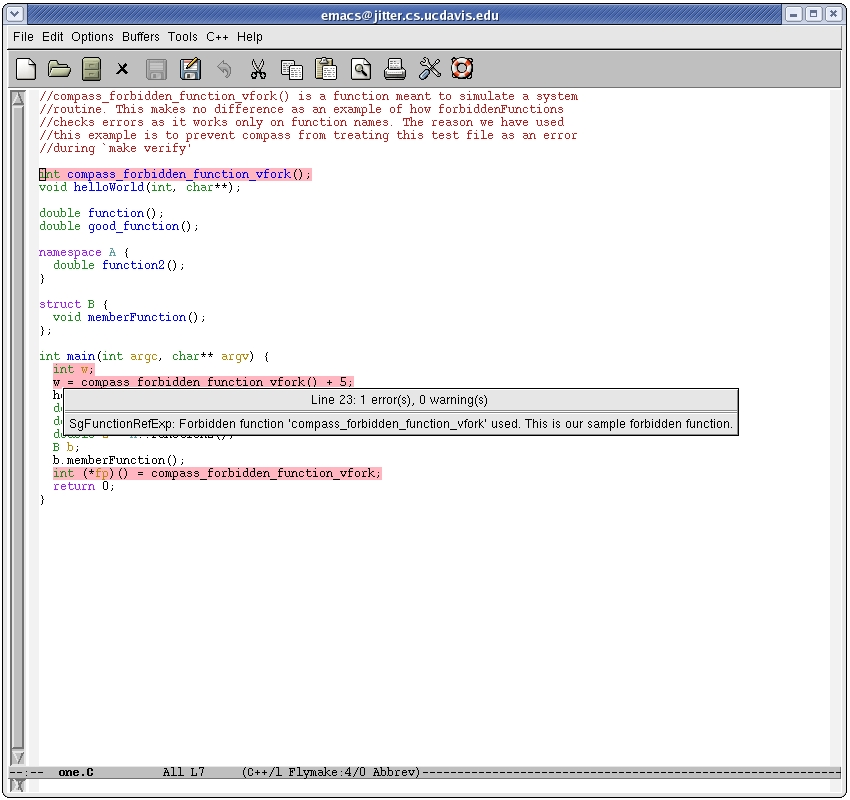
\includegraphics[width=7in]{emacs_screenshot.jpg}
\caption{Compass error messages integrated into Emacs}
\label{Compass_Emacs_Screenshot}
\end{figure}

\begin{figure}
%\center
\hspace{-1.35in}
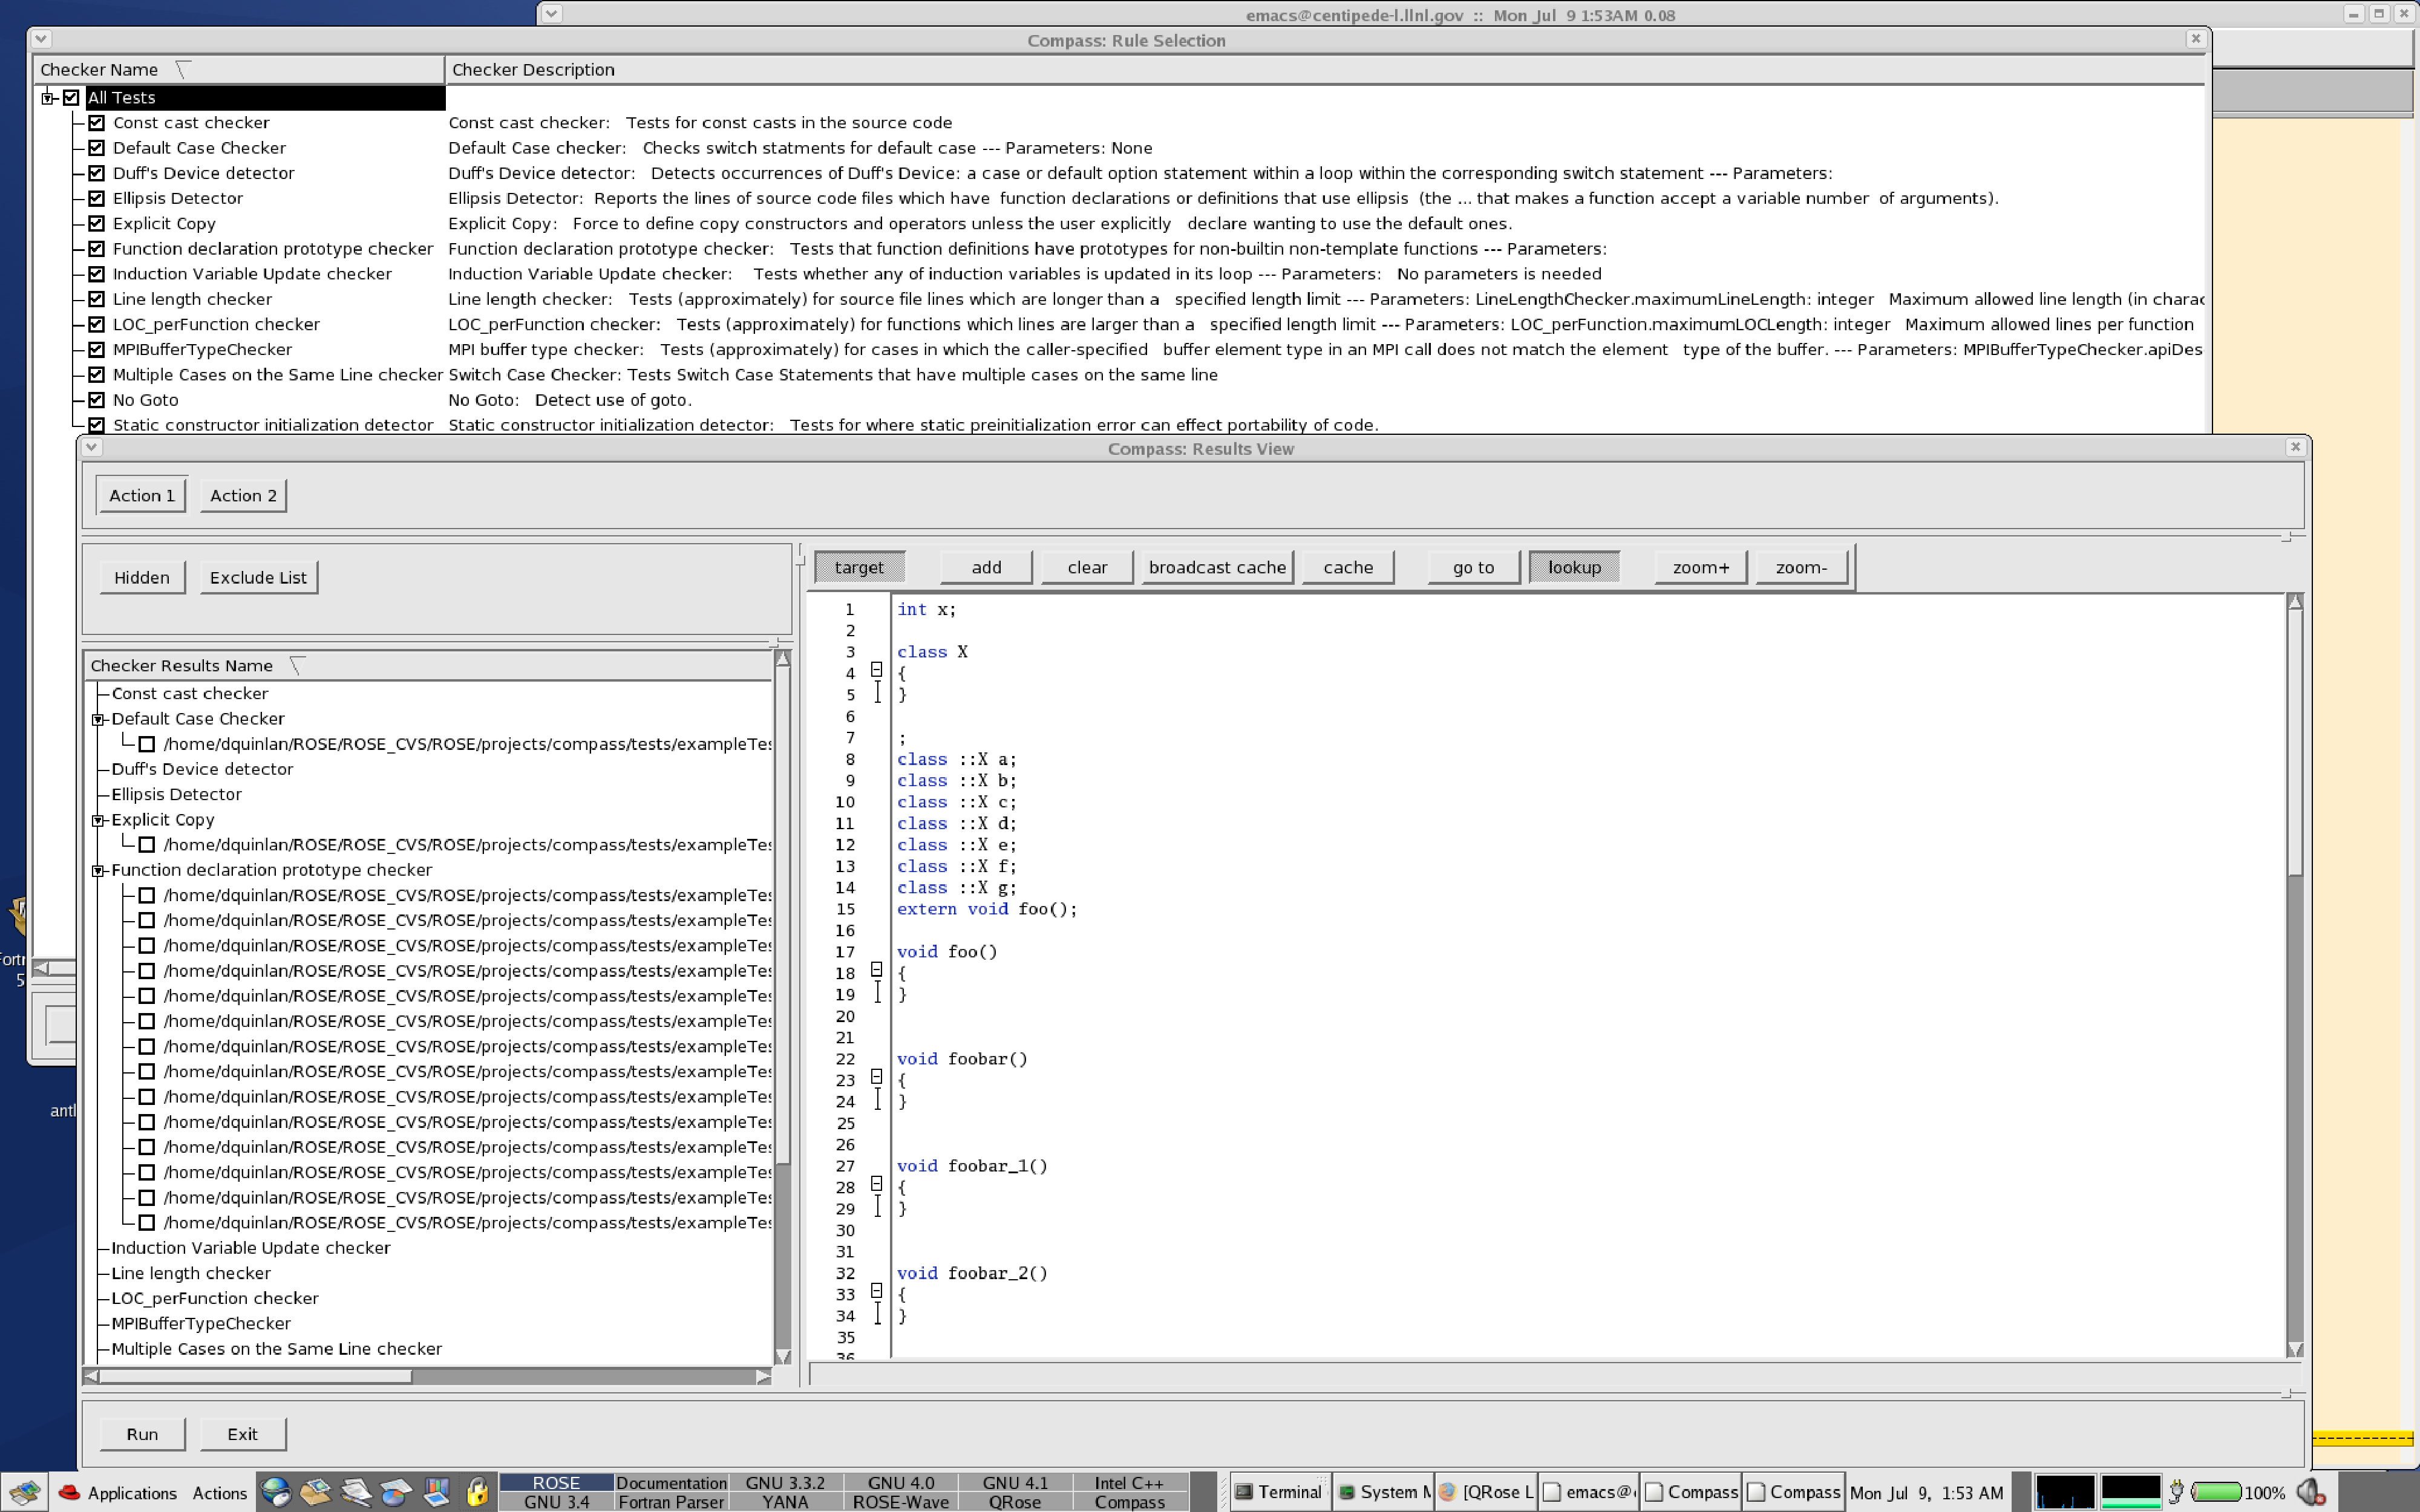
\includegraphics[width=7in]{CompassScreenshot.pdf}
\caption{Compass GUI for interpretation of rule violations}
\label{Compass_GUI}
\end{figure}

\begin{figure}
\hspace{-0.7in}
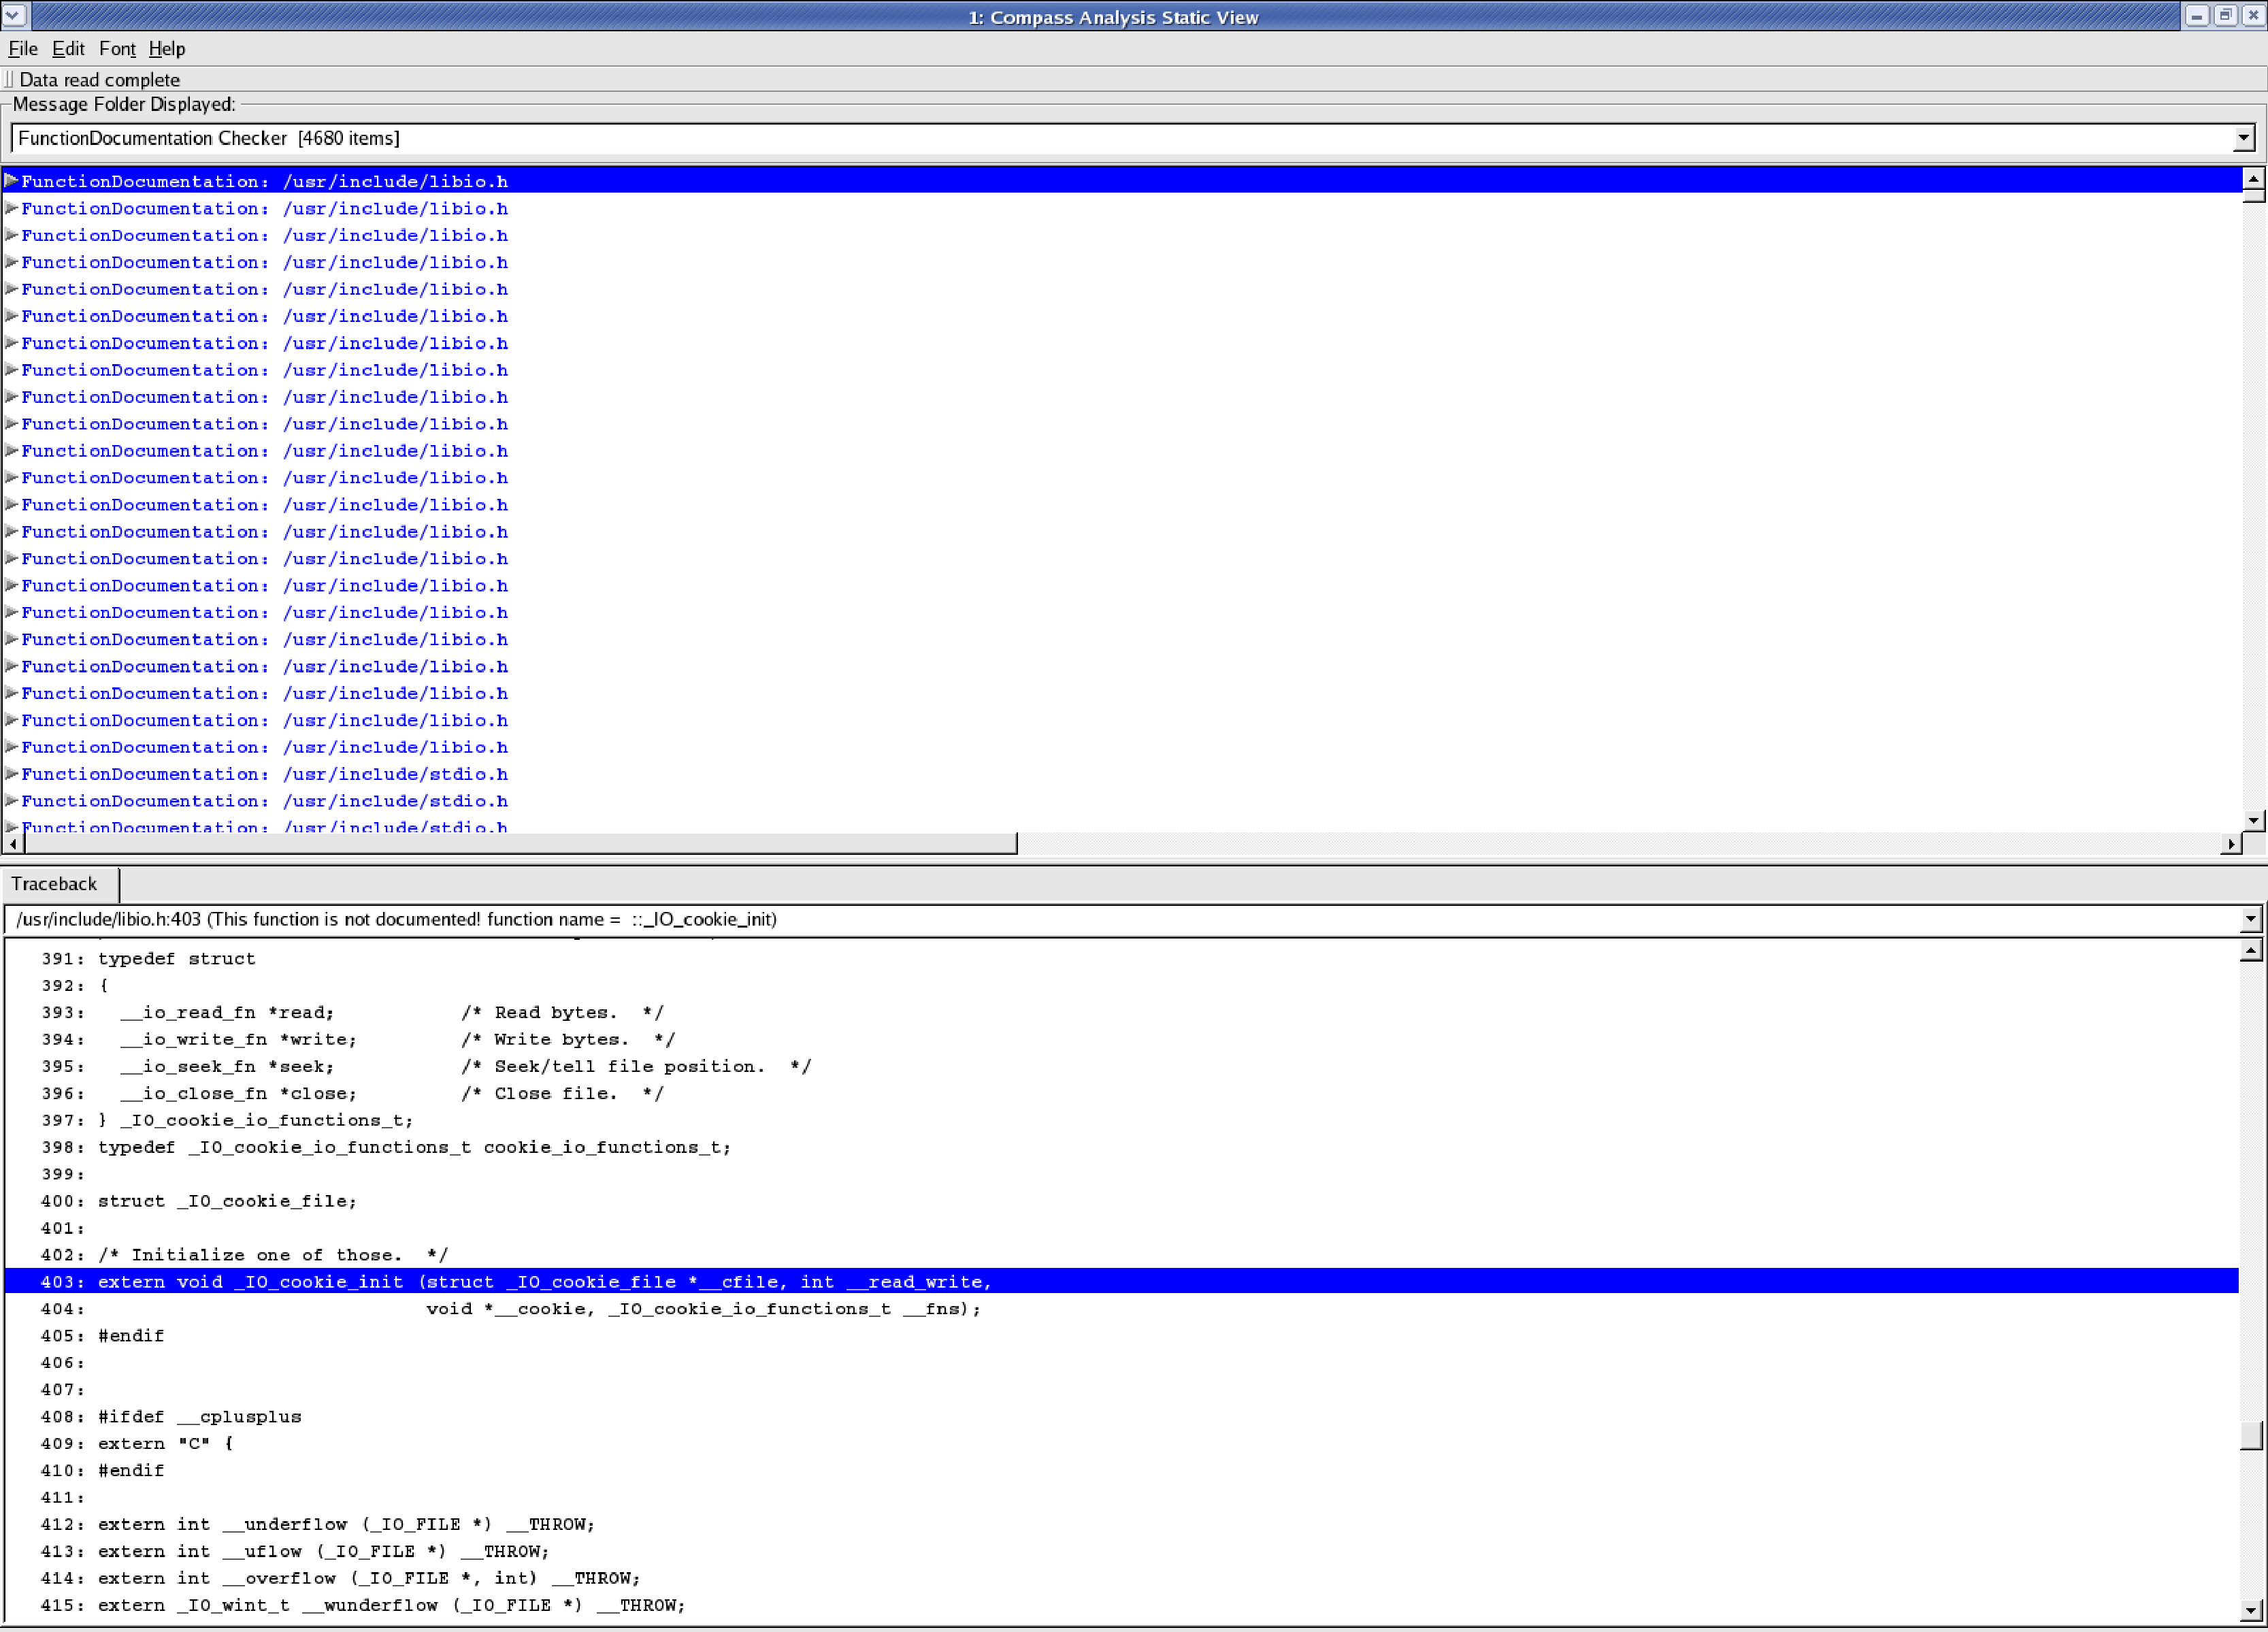
\includegraphics[width=7in]{ToolGear_gui_compass_01.pdf}
\caption{Processing of XML Compass output using ToolGear}
\label{Compass_ToolGear_Screenshot}
\end{figure}

\begin{figure}
{\scriptsize
\begin{verbatim}
LocalizedVariables: /home/ROSE/projects/compass/tests/Cxx_tests/test2006_117.C:30.5: Variable pmNull does not seem to be used.
FunctionDefinitionPrototype: /home/ROSE/projects/compass/tests/Cxx_tests/test2006_123.C:27.1-10: matching function prototype not available
LocPerFunction: /home/ROSE/projects/compass/tests/Cxx_tests/test2006_117.C:23.1-20: This function has too many lines of code :: LOC = 14 > 10
MagicNumber: /home/ROSE/projects/compass/tests/Cxx_tests/test2006_117.C:33.14: Occurrence of integer or floating constant.
MagicNumber: /home/ROSE/projects/compass/tests/Cxx_tests/test2006_117.C:36.14: Occurrence of integer or floating constant.
MagicNumber: /home/ROSE/projects/compass/tests/Cxx_tests/test2006_117.C:37.14: Occurrence of integer or floating constant.
FunctionDocumentation: /home/ROSE/projects/compass/tests/Cxx_tests/test2006_123.C:27.1-10: function is not documented: name =  ::main
FunctionDocumentation: /home/ROSE/projects/compass/tests/Cxx_tests/test2006_123.C:9.10: function is not documented: name =  ::X < int , int , 10 > ::f
FunctionDocumentation: /home/ROSE/projects/compass/tests/Cxx_tests/test2006_123.C:12.10: function is not documented: name =  ::X < int , int * , 5 > ::f
FunctionDocumentation: /home/ROSE/projects/compass/tests/Cxx_tests/test2006_123.C:16.10: function is not documented: name =  ::X < int * , float , 10 > ::f
\end{verbatim}
}
\caption{Example of ASCII output from Compass. }
\label{Compass_ASCII_Output}
\end{figure}



\subsection{Using Compass With Emacs}

\label{compass::emacs}

Compass as a checker is most useful when the user is notified as early as possible
when he violates a desired software property. Although for many purposes it is
sufficient to run Compass separately; it is possible to use compass
seamlessly when developing in emacs. By using an emacs extension called {\em flymake} together
with Compass erroneous lines can be highlighted while programming, and the relevant error messages displayed 
in a dialog. Syntax errors from ROSE will be displayed as well, see figure \ref{Compass_Emacs_Screenshot}.

Much thanks for David Svoboda at CERT at CMU for first configuring Flymake to work with
Compass and demonstrating the idea.  It has provided a great way to check code using
compass and its use in Emacs has stimulate a number of ideas that have made their way
back into Compass.

\subsubsection{Emacs .emacs Code Requirement}

   Figure \ref{compassEmacs} shows the code that is required to be added to the {\tt .emacs}
file.  A copy of this code is available in the compass source directory in the file
{\tt emacs\_compass\_config.el}.

\begin{figure}
{\scriptsize
\begin{verbatim}
; New Compass support for Emacs using version 22 of Emacs and Flymake.
; Comment out these two lines to use older version of emacs.
(require 'flymake)
(setq flymake-allowed-file-name-masks (cons '(".+\\.C\\'" flymake-simple-make-init flymake-simple-cleanup flymake-get-real-file-name) flymake-allowed-file-name-masks))


(defun flymake-master-make-header-init ()
  (flymake-master-make-init 'flymake-get-include-dirs
			    '("\\.C\\'" "\\.c\\'")
			    "[ \t]*#[ \t]*include[ \t]*\"\\([[:word:]0-9/\\_.]*%s\\)\""))

(add-hook 'find-file-hook 'flymake-find-file-hook)

(setq flymake-log-level 3)
(setq flymake-no-changes-timeout 0.5)

(defcustom rose-source-tree "/home/dquinlan/ROSE/NEW_ROSE/" "Location of top of ROSE source tree")
(defcustom rose-build-tree "/home/dquinlan/ROSE/ROSE_CompileTree/LINUX-64bit-3.4.6/" "Location of top of ROSE build tree")
(defun add-buildfile-dir-for-rose ()
  (let ((source-dir-name (file-name-directory buffer-file-name)))
    ;(message "%S" `(source dir ,source-dir-name))
    (if
      ; (string-equal rose-source-tree (substring source-dir-name 0 (length rose-source-tree)))
        (string-equal rose-source-tree (substring source-dir-name 0 (min (length source-dir-name) (length rose-source-tree))))
        (let ((buildfile-dir (concat "../../../../../../../../../../../../../../../../../../../" rose-build-tree "/" (substring source-dir-name (length rose-source-tree)))))
        ; (message "%S" `(buildfile-dir ,buildfile-dir))
        ; (set-variable 'flymake-buildfile-dirs (cons buildfile-dir flymake-buildfile-dirs) 'local))
          (set-variable 'flymake-buildfile-dirs (append (mapcar (lambda (dir) (concat buildfile-dir "/" dir)) flymake-buildfile-dirs) flymake-buildfile-dirs) 'local))
      (progn
        ;(message "%S" `(bad-prefix))
        source-dir-name))))
(defun set-rose-source-dir (dir) "Set the top of the ROSE source tree to use with Flymake" (interactive "DThe top of the ROSE source tree: \n")
  (setq rose-source-tree dir 'local)
  (add-buildfile-dir-for-rose))
(defun set-rose-build-dir (dir) "Set the top of the ROSE build tree to use with Flymake" (interactive "DThe top of the ROSE build tree: \n")
  (setq rose-build-tree dir 'local)
  (add-buildfile-dir-for-rose))

(add-hook 'find-file-hook 'add-buildfile-dir-for-rose)

;(list "make"
;;  (list "-s" "-C" "/home/dquinlan/ROSE/NEW_ROSE/developersScratchSpace/Dan/EmacsCompass_tests/"
;    (list "-s"
;   (list "-s -C" "`pwd | sed 's@^/home/dquinlan/ROSE/NEW_ROSE/@/home/dquinlan/ROSE/ROSE_CompileTree/LINUX-64bit-3.4.6/@'`"
;	   (concat "CHK_SOURCES=" source)
;	     "SYNTAX_CHECK_MODE=1"
;		   "check-syntax"))

(global-set-key [f3] 'flymake-display-err-menu-for-current-line)
(global-set-key [f4] 'flymake-goto-next-error)

\end{verbatim}
}
\caption{Addition to .emacs when integrating Compass into emacs. }
\label{compassEmacs}
\end{figure}

\subsubsection{Emacs Version Requirement}

Emacs version 22 or newer is required to take advantage of the emacs integration of
Compass. Before using Compass a 3 step process must be followed:
\begin{itemize}
   \item Add the text in figure \ref{compassEmacs} (in \\*{\tt ROSE/AUG0508/ROSE/projects/compass/tools/compass/emacs\_compass\_config.el}) to .emacs
   \item Change /path/to/makefile in figure \ref{compassEmacs} to the path to the project you are editing in Compass
   \item Add a 'check-syntax' rule to the makefile of the project that you are working
   on in Compass. This rule should compile all the files you want Compass to check 
   or all files that you are editing with Compass as the compiler.
\end{itemize}

Figure \ref{compassEmacs} shows the needed changes in .emacs for integrating
Compass. The last two lines are the most interesting lines since they introduce two
shortkeys. [f3] can be clicked in order to display all errors for the current line while
[f4] will move the cursor to the next error. 

A short explanation of the code in figure \ref{compassEmacs} is that the first line will require 
the flymake extension to be available upon
loading emacs while the second line will load the find-file-hook and flymake-find-file-hook
functions. The "setq" sections that follows runs Compass for all files that are being edited
that has the c and C extensions. The ``list'' section tells flymake to execute the check-syntax
rule in the makefile. 

\subsubsection{Example check-syntax rule}


\begin{figure}
\begin{verbatim}
one: inc.h one.C
        g++ -c one.C
\end{verbatim}
\caption{Example makefile before the Compass addition  }
\label{beforeProjectCheckRule}
\end{figure}


\begin{figure}
\begin{verbatim}
one: inc.h one.C
        g++ -c one.C
		
check-syntax: inc.h one.C
        /path/to/compass/executable/compassMain -c one.C
\end{verbatim}
\caption{Example makefile after addition to support integration of compass  }
\label{projectCheckRule}
\end{figure}


Figure \ref{beforeProjectCheckRule} shows an example makefile that compiles a file
"one.C" using g++. If "one.C" is edited using emacs the addition of the "check-syntax"
rule is needed, as shown in figure \ref{projectCheckRule}.

\subsection {Using Compass With Vim}
%--------------------------------------------
Compass can be used with Vim 7's QuickFix commands to display warning
messages and highlight the source lines in question. A compass compiler
plugin (compass.vim as shown in Figure \ref{compassVim7})  has
been provided for Vim to parse the warning messages outputted by Compass.

Steps to make Compass work with Vim 7
\begin{itemize}
\item Save compass.vim into ~.vim/compiler.  Create the target directory if it
does not exist.
\item Download errormarker.vim from
http://www.vim.org/scripts/script.php?script\_id=1861 and save it
into .vim/plugin . Again, create the target directory first when it does not
exist.
\item Change your Makefile to use an installed compassMain as the compiler
to compile your code.
\item Use quickfix features of Vim 7 as documented at
http://vimdoc.sourceforge.net/htmldoc/quickfix.html. Some frequently used
commands are:
  \begin{itemize}
   \item Specifying the compass plugin to use by typing a command :compiler compass
   \item Open your source code using gvim and set the compiler to Compass by
   \item Compile you code using compassMain, type :make
   \item Display current message, type :cc
   \item Display all messages, type :clist
   \item Jump to next message, type :cnext
  \end{itemize}
\end{itemize}
%-------------------------------
\begin{figure}[!htp]
{\scriptsize
\begin{verbatim}
" Vim compiler file
" Compiler:     ROSE Compass 0.9.2a
" Maintainer:   Chunhua Liao <youraccount@llnl.gov>
" Last Change:  2008 Apr. 3
"
if exists("current_compiler")
  finish
endif
let current_compiler = "compass"

if exists(":CompilerSet") != 2          " older Vim always used :setlocal
  command -nargs=* CompilerSet setlocal <args>
endif

" single line warning
" multiple line warning, %W, %C continue line %Z end of multiple line
CompilerSet errorformat=%s:\ %f:%l%.%c:\ %m,
         \%s:\ %f:%l%.%c-%*\\d:\ %m,
         \%s:\ %f:%l%.%c-%*\\d%.%*\\d:\ %m,
         \\\"%f\"\\,\ line\ %l%*\\D%c%*[^\ ]\ %m
"some notes about the error/warning message format
"Official guide: http://vimdoc.sourceforge.net/htmldoc/quickfix.html#error-file-format
" Each new rule start with a leading \ unless it is the first rule in the
" first line
"  %f: filename %l: line number %c: column number, only one is permitted %m
" actual error/warning message \ :matching a space
"  %*\\d: matching any number

\end{verbatim}
}
\caption{A compiler plugin for Vim 7 compass.vim}
\label{compassVim7}
\end{figure}
%-------------------------------
Figure ~\ref{Compass_VIM7_Screenshot} shows an example of Compass error
messages integrated into Vim 7.
\begin{figure}[!htp]
%\centering
\hspace{-0.7in}
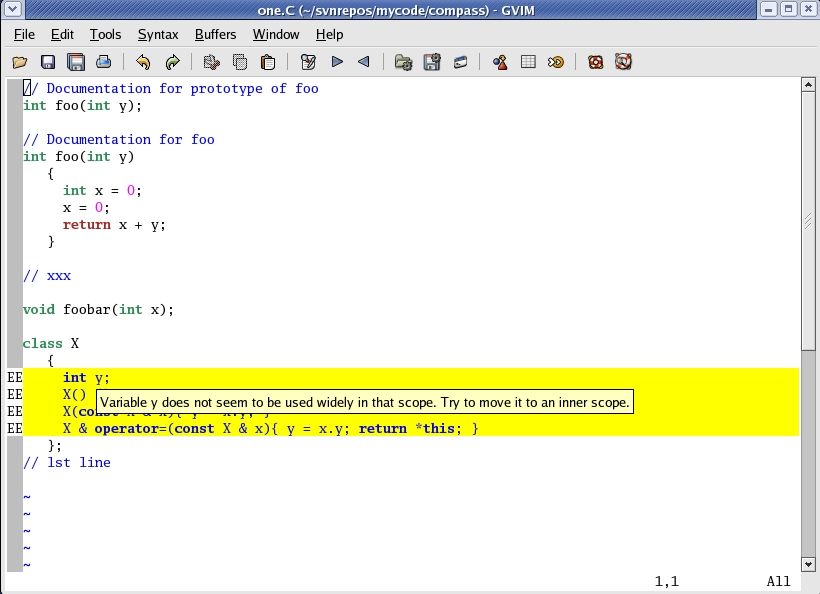
\includegraphics[width=7in]{compass_vim7.jpg}
%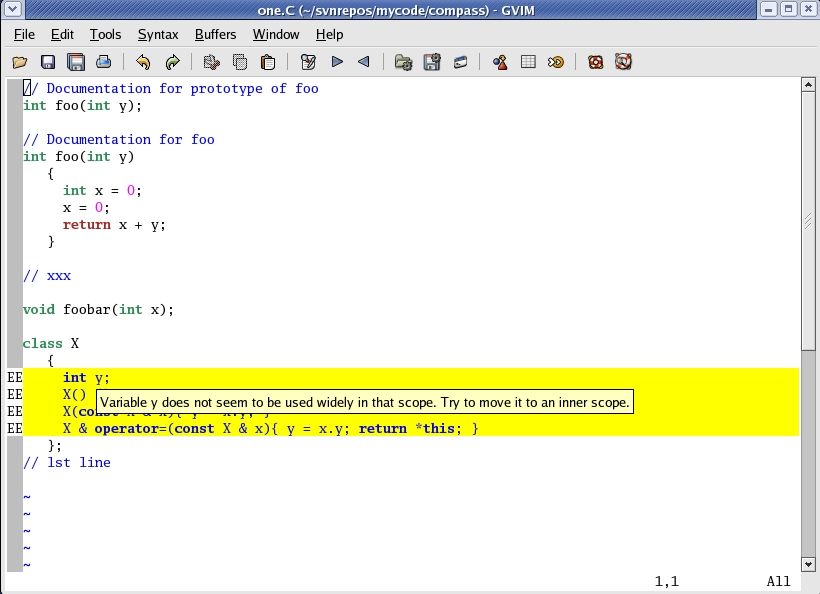
\includegraphics[width=0.7\textwidth]{compass_vim7.jpg}
\caption{Compass error messages integrated into Vim 7}
\label{Compass_VIM7_Screenshot}
\end{figure}


\section{Including/Excluding Checkers in the Compass Build Process}
\label{CompassBuildProcess}

   This section describes how to select which of the checkers to integrate 
into Compass out of all the checkers available in source form in the Compass 
source directory. For security reasons Compass uses this static build process 
since it is a central goal of Compass that it should run as a trusted part of 
a project's build process. If the integration of checkers had been automatic 
through a dynamic plugin mechanism it would be hard to ensure that the dynamic 
list of checkers was secure, but for a static list of trusted checkers this is 
possible.

The file ROSE\_SOURCE\_DIR/projects/compass/tools/compass/CHECKER\_LIST is used to control which checkers are selected to
be compiled into compassMain. It can use the `\#' comment delimiter at the beginning of
any checker name to remove that checker from compilation. The hash mark may
only appear at the beginning of the line. The compass\_submission\_setup.sh
script must be run again with the ``regenerate'' option if any checkers are
commented out. 
{\bf Note that no space is permitted between the `\#' and the name
of the checker.}

Usually the CHECKER\_LIST is only modified when a user or developer wants to 
add a new checker or select a subset of trusted checkers.  Checkers can be
commented out using a {\tt \#}, no space is allowed between the {\tt \#} 
and the checker name.

\section{Including/Excluding Checkers During Compass Execution}
\label{ruleselection}

   This section describes how to execute a subset of the checkers provided in the build
process (see section \ref{CompassBuildProcess}). This process is significantly more
interactive than defining what checkers to include in the Compass build process.
Since it is not unheard of that rules implemented by different checkers can be  
mutually exclusive or even contradicting this mechanism is essential for selecting the
subset of checkers that are interesting for a specific program that is checked.
Separate projects of developers could easily have their own RULE\_SELECTION file
to permit high levels of customization in the use of a Compass tool containing
a large number of checkers (e.g. for different languages).

   When used with the Emacs interface this provides a simple way to turn on and off
specific checkers by editing a single file (RULE\_SELECTION).  The name of this
file is specified in the {\tt compass\_parameters} file, this name may be changed.
The directories searched are: current directory, user home directory, and Compass
source tree (respectively). \fixme{The current implementation may not
support all of the mentioned search paths.}

\begin{verbatim}
   Compass.RuleSelection=/path/to/your/RULE_SELECTION
\end{verbatim}

In order to select a checker to run the user must:
\begin{itemize}
   \item Add a line '-:$<$name of checker$>$' in a file called RULE\_SELECTION. 
   \item If a line  '-:$<$name of checker$>$' already exist the '-' can be modified into
a '+' to enable the checker or into a '-' to disable a checker.
\end{itemize}
It is required that every checker integrated into the Compass build is mentioned in
the RULE\_SELECTION.


\section{Including/Excluding Paths and Filenames with Compass}

    Compass permits paths and filenames to be specified for inclusion/exclusion
in reporting checker rule violations.  Run {\tt compassMain --help} to see
the commandline options.  Numerous other commandline options provided for all
tools build using ROSE may also be relevant.



\section{Checking Security Properties of Checkers}
\label{sec:compass_verify}

    Compass is designed for extensibility while providing the security for
the codes being checked.  To support this Compass provides a simple
mechanism for verifying specific properties of the checkers used in Compass.
Compass implements a specific small number of checkers that are used for checking
the checkers in Compass.  The directory compassVerify contains the implementation
of this subset of Compass that is used on itself.  These checkers may not
be modified and in the future MD-5 checksums will be provided to ensure the
integrity of this subset of Compass.  To verify the compass checkers run:
\begin{itemize}
   \item {\tt make verify} \\
        This makefile rule runs the compassVerify/compassMain on all the source files in
    all the checkers directories in Compass.  Because it runs compass on so
    many separate
    files this step can take a long time.
   \item Or {\tt make oneBigVerify} \\
        The makefile rule runs the compassVerify/compassMain on a single generated file
    built from all the checker source files and is particularly quick to run.
\end{itemize}



\section{Testing Compass and its Checkers}

   The {\tt tests} directory contains directories of tests that
are language specific:
\begin{itemize}
   \item C\_tests \\ 
         This directory contains a Makefile which will use the ROSE C test codes 
         to test Compass.
   \item Cxx\_tests \\ 
         This directory contains a Makefile which will use the ROSE C++ test codes 
         to test Compass.
\end{itemize}
To run these tests type {\tt make check} at any level on the Compass directory
hierarchy of the build tree.
%-------------------------------
\clearpage
\section{How To Write A New Checker}

\subsection{Creating A Skeleton}

Compass has scripts for creating a skeleton for a new Compass
checker. This skeleton can be easily adapted to write all checkers.

Follow these steps to generate a checker skeleton:
\begin{enumerate}
   \item Enter a directory where you want the directory of your checker to
   be created: For example,
   rosesourcetree/projects/compass/extensions/checkers.
   \item Execute {\tt
   ROSE\_SRC\_DIR/projects/compass/src/compass\_scripts/gen\_checker.sh
   $<$name of your checker$>$} (the name of your checker can have space and
   the script will automatically concatenate them to camel case, e.g: 
   "multiple case on same line")
\end{enumerate}

The results of executing gen\_checker.sh script is that a new directory name 
``multipleCasesOnSameLine''
(name of your checker in camel case) is created with the following files:
\begin{itemize}
\item compass\_parameters : internal parameters for this checker 
\item multipleCasesOnSameLine.C : main source file 
\item multipleCasesOnSameLine.compass.external.makefile : makefile if this
checker is to be built outside of the ROSE source tree.
\item multipleCasesOnSameLineDocs.tex : documentation 
\item multipleCasesOnSameLine.inc : Makefile include file
\item multipleCasesOnSameLine.h : header
\item multipleCasesOnSameLineMain.C : main driver
\item multipleCasesOnSameLineTest1.C : test input code
\end{itemize}

Some of these files (compass\_parameters)
are copied from the compass\_template\_generator directory; while others are
generated (multiple*, *.makefile)

It is suggested that you keep the following in mind when using gen\_checker.sh:
\begin{itemize}
\item
   It is advised that you do not invoke the script gen\_checker with words
   like checker, detector, tester, etc. Adding these verbs at the command
   line means that these words are added as suffixes into the
   directory-name. Which will make it redundant, as the compass project is
   about writing style-checkers!
\item
   Some of the files\fixme{What are the readonly files exactly?} have read-only permissions and are intended only for
   such use. Please do not change the permissions of these files.
%\item
%Advanced: The file `multipleCasesOnSameLine.inc' is used to pass in custom LDADD lines
%to the Make environment on a per checker basis. The LDADD line specified in
%this file will be added verbatim to the compass makefile.

\end{itemize}

\subsection{Integrating New Checkers Into Compass Tool}
\label{howToIntegrateNewCheckers}

The process for integrating a new checker into Compass has been automated. 
These directions are meant for checkers generated using gen\_checker.sh. 
The process is similar for all compass-like tools that are built using the 
common infrastructure.

The steps to integrate a new checker is (note that both of the source tree and
build tree of ROSE are involved):
\begin{enumerate}
   \item Add $<$camel case of your checker name $>$ to
   ROSE\_SOURCE\_DIR/projects/compass/tools/compass/CHECKER\_LIST
   \item Enter ROSE\_BUILD\_DIR/projects/compass/tools/compass
   \item Execute 'make regenerate'
   \item After running 'make regenerate' in the build tree then you may run make as usual.
   \item Examine the ROSE\_SOURCE\_DIR/projects/compass/tools/compass/RULE\_SELECTION.in file and confirm it
	reflects your most recent additional checker(s) choice of execution at
	run-time; the default setting is ``on''. Please refer to section 
	~\ref{ruleselection}.
\end{enumerate}

% Typing make testNewChecker manually will cause later make check fail
% Not recommended to use, Liao, 10/31/2008
%Additionally, a blank checker may be automatically integrated into the current
%compass tool as a method to test for build system errors. To execute this test
%,type:
%
%\begin{verbatim}
%make testNewChecker
%\end{verbatim}
%
%from any compass tool directory. This test will create a blank checker from
%the template attempt to install the checker then uninstall it thus leaving the
%tool in its previous state.

%Many automatically generated files required for the build of Compass are 
%generated in the build tree. Rules for the generation of these files are found
%in the automake Makefile.am file in the Compass source tree directory 
%projects/compass. These file include:
%
%\begin{itemize}
%\item {\bf CHECKER\_LIST\_WITHOUT\_COMMENTS}: a version of CHECKER\_LIST
%	that expands in two columns those checkers built as part of Compass
%	in camel case starting with a lower-case letter and an upper-case
%	letter respectively.
%
%\item {\bf checkers.h}: An automatically generated file needed by compassMain.C that 
%	contains a list of \#include directives for each checker header .h file.
%
%\item {\bf buildCheckers.C}: An automatically generated source file needed by 
%	compassMain.C to build the Compass checker traversals.
%
%\item {\bf compass\_parameters}: The concatenation of individual checker parameter files to be used with compassMain.
%
%\item {\bf testNewChecker}: creates a blank checker from the template and
%	attempts to automatically install it into the current compass tool then
%	uninstall it again. This label is used to test the build system.
%
%\end{itemize}




\section{Extending the Compass Infrastructure}

Compass, as well as being a tool for software analysis, is also a capable
infrastructure for building other tools like Compass that utilizes the work
put into Compass checkers. There are many reasons why one would like to have 
a separate executable tool beneath Compass rather than simply customizing a
particular build of the Compass tool. An individual or organization may
consider a specific subset of Compass checker rules to be particularly
relevant; thus would like to have a custom tool to check only these rules.
Another scenario may find that the particular interface for Compass through
the command line needs to be changed; but, it is not advisable to alter
Compass main directly!

This section will demonstrate how to extend the Compass
infrastructure and checkers to build a separate executable tool beneath
the Compass project. A simple tutorial will detail the steps necessary
to instantiate the Compass infrastructure. The these steps have been
followed and the mechanism is demonstrated in an example directory 
({\tt sampleCompassSubset}; this directory can be copied.

Suppose one wishes to build a version of Compass with only those checker rules
authored by an individual for debugging purposes. Certainly, it would not
be desirable for the main Compass tool to only consist of this subset of rules; yet
this specialized version might be required regularly enough for repeatedly altering
of the static or dynamic checker rule selection files to become troublesome.
The solution is to use the Compass infrstructure to build a separate tool
by creating a subdirectory under Compass with a small portion of Compass 
infrastructure files. Only four files are required: compassMain.C, CHECKER\_LIST,
RULE\_SELECTION, Makefile.am.  Note also that the {\tt compassMain.C} file
can be any name, but must only be consistant with the {\tt Makefile.am}. This
example of using the compass infrastructure is compiled as part of compiling
compass and defines a compass-infrastructure-based tool that implements
about 25 randomly selected checkers (form the collection in {\tt projects/compass/extensions/checkers}).

Assume that the present working directory is {\tt projects/compass/tools} 
of the ROSE source tree. First, create a directory for the new Compass 
subset tool.
%
\begin{verbatim}
mkdir sampleCompassSubset
\end{verbatim}
%
then add this directory in the {\tt SUBDIRS} variable of the automake file
{\tt projects/compass/tools/Makefile.am}. Additionally, introduce this new 
Makefile into the top level source tree {\tt configure.in} file. A snippet 
concerning these changes is given below:
%
\begin{verbatim}
projects/compass/tools/Makefile.am:
SUBDIRS = compass compassVerifier sampleCompassSubset
\end{verbatim}
%
\begin{verbatim}
configure.in:
projects/compass/tools/sampleCompassSubset/Makefile
projects/compass/tools/compassVerifier/Makefile
\end{verbatim}
%
{\it Note that after any modification of {\tt configure.in}, the configure command
for ROSE will have to be rerun (else the makefile will cause it to be called
for you).}

\vspace{0.2in}

To specify how this tool is to be configured and built create a 
{\tt Makefile.am},
{\tt projects/compass/tools/sampleCompassSubset/Makefile.am} is provided as an 
example.
This example can be a template and may be used in general for any Compass-like 
tool.
Any tool that is an extension of the Compass infrastructure will reuse much of 
the Compass infrastructure such as {\tt compassSupport}.
Furthermore, much of the Compass build
process requires the automatic generation of files in the build tree such
as {\tt compass\_makefile.inc}, {\tt compass\_parameters}, etc. Thus an
include file has been provided in Compass to define these common rules--
{\tt compass.inc}; and is included in this {\tt Makefile.am}.
A more advanced implementation of this automake file template is located in
Compass Verifier; which is itself another tool extended off Compass and
designed to check the rules implemented in Compass.

So far, a blank Compass-like tool has been created and configured to build with
ROSE. Still missing are a few Compass files that produce a successful
compile and linked executable. The next step is to populate the empty 
Compass-like tool with checkers from Compass. Note that all checkers
reside as subdirectories in {\tt projects/compass/extensions/checkers};
but that subsets of
these are selected for use, thus all checkers are always optionally available 
to all compass-infrastructure-based tools.  Create a new file called
{\tt CHECKER\_LIST} under the {\tt sampleCompassSubset} directory (an
example has been provided) and insert the names of the desired checkers into
this file. One may also create the dynamic rule selection file 
{\tt RULE\_SELECTION} or defer this file to be automatically generated with
all checker rules activated by default. Finally, it is necessary to write or
copy the {\tt compassMain.C} file that defines (among other function)
the command line processing options where one may alter the interface. 
For {\tt sampleCompassSubset} the {\tt compassMain.C} of 
{\tt projects/compass/src/compassSupport} 
is symbolically linked in place. The complete directory list for 
{\tt sampleCompassSubset} now looks like

\begin{verbatim}
CHECKER_LIST
compassMain.C -> ../../src/compassSupport/compassMain.C
Makefile.am
RULE_SELECTION
\end{verbatim}

The source tree creation and configuration of a new Compass-like tool is 
complete with {\tt Makefile.am}, {\tt CHECKER\_LIST}, {\tt RULE\_SELECTION},
and {\tt compassMain.C} (rename {\tt compassMain.C} as you like just make
sure that the name is consistant with the {\tt Makefile.am}). Build and 
configure ROSE as usual and then invoke Make at the top level build tree 
or {\tt projects/compass} subdirectory to
compile and link the new Compass-like tool executable. In this tutorial 
example the new target location is 
{\tt projects/compass/tools/sampleCompassSubset}.


\newpage

\chapter{Using Compass GUI}

Compass has a GUI available for exploring the checker warnings for either the compilation
of a single source file or the compilation of a whole project. This GUI allow the user to
interactively select checkers, run those checkers on the source file(s) of 
interest and display the source location of each violation. As a user convenience the
interface will either display the violating source region in a text editor or a 
non-editable display window.

The Compass GUI is located in the 'projects/compass/tools/compass/gui' directory of the
ROSE distribution. The Compass GUI is build as part of the standard Compass build when
ROSE is configured with qt4. In order to enable simple compilation of whole projects using
one-button clicks in the Compass GUI ROSE must be configured with sqlite3 as well.

\section{Running Compass GUI on a Single File}
\label{runningCompassGUISingleFile}

Before running the Compass GUI on a single file  the files listed 
in \ref{usingCompassInstallation} must be available and the environment variable 
'\$COMPASS\_PARAMETERS' must specify which compass\_paramaters file to use. CompassGUI can
then be invoked as a normal compiler like e.g:
\begin{verbatim}
compassMainGui -o ex1 ex1.C
\end{verbatim}
If it is not desirable to export the '\$COMPASS\_PARAMETERS' variable a shorthand is:
\begin{verbatim}
env COMPASS_PARAMETERS=/location/of/compass_pramateres   compassMainGui -o ex1 ex1.C
\end{verbatim}

\section{Running Compass GUI on an Autotools Project}

A goal of this section is to show how to run the compass checkers on a whole project (like e.g ROSE) 
using a one button click in the Compass GUI and present an easy interface for exploring the violations
as found during the build. This interface is currently limited to sequentially building the
project and it requires ROSE to be configured with sqlite3. The Compass GUI does not try to replace the 
build system; it simply captures how the build system compiles the source files for a specific version of the 
project. Although there is no guarantee that this will work when the source code changes it is reasonable to 
expect the capturing of the build system should be the same as the code evolves as long as no changes are done 
to the build system.

These instructions can apply to Autotool projects as well as projects build in other build 
systems, but the shorthands used here for discerning the build system are specific for Autotools.


\subsection{Capturing a Build System State}

\fixme{Document: that this requires --with-sqlite3}

The first step of running the Compass GUI on an autotools project is to figure out how the build system
works. Capturing the build system state is done with the 'buildInterpreter' tool provided in the Compass
distribution in the 'projects/compass/tools/compass/buildInterpreter' directory. 

In order to facilitate capturing the build system once and moving the source files around the '\$ROSE\_TEST\_REGRESSION\_ROOT' environment variable must be defined to the string that should be replaced. For instance if a
projects is build within /home/user/project and it is desired to move the files inside that directoy to a
different directory define it to be
\begin{verbatim}
export ROSE_TEST_REGRESSION_ROOT=/home/user/project
\end{verbatim}

\fixme{Document: Need to be in the buildInterpreter directory.}

The buildInterpreter tool works as a replacement for the C/C++ compiler during compilation like e.g:
\begin{verbatim}
buildInterpreter -o ex1 ex1.C
\end{verbatim}
The output of the run is a database representing how to compile ex1.C. The name of the output database is specified
by the 'dbname' field in the rqmc file found in the ROSE build directory under 'projects/compass/tools/compass/buildInterpreter/rqmc' and defaults to 'test.db'.

To capture the state of a whole build system use 'buildInterpreter' as a replacement for the C/C++ compiler during
the build. E.g for gnu make:
\begin{verbatim}
make CC=buildInterpreter CXX=buildInterpreter
\end{verbatim}

\subsection{Build A Project Using the Discerned Build }

To build a project using Compass specify the output database from the capturing of the build state with the
'--outputDb' paramater to the Compass GUI. The environment variable must be defined like in \ref{runningCompassGUISingleFile}, e.g:
\begin{verbatim}
cd /directory/with/build/project/sources
env COMPASS_PARAMETERS=/location/of/compass_pramateres   /compass/gui/build/compassMainGui --outputDb test.db
\end{verbatim}
In the GUI click on regenerate to build the project. The violations found during the build is put into the database
for subsequent lookup. After regenerating select the checkers that you are interested and and click 'refresh' to display the corresponding violations.






\newpage

%%%%%%%%%%%%%%%%%%%%%%%%%%%%%%%%%%%%%%%%%%%%%%%%%%%%%%%%%%%%%%%%%%%%%%%%%%%%%%%%
%
%
%
%%%%%%%%%%%%%%%%%%%%%%%%%%%%%%%%%%%%%%%%%%%%%%%%%%%%%%%%%%%%%%%%%%%%%%%%%%%%%%%%

\chapter{Using Compass Verifier}

	Compass Verifier is a tool extended from Compass to analyze the source
code of Compass and its checkers to detect certain properties. The motivation
and design of this tool are discussed in Chapter 2 (Design and Verification).
This chapter will detail the Make rules written to run Compass 
Verifier and to setup the parameters to the AllowedFunctions checker.

The rules to setup and run Compass Verifier are found in 
{\tt projects/compass/tools/compassVerifier/Makefile.am}. Follows is an 
overview of their usage labels, ({\tt make oneBigVerify, verify, ...}).
Verifier is designed to examine the compass tool referenced in the environment
variable {\tt \$(TOOLBUILD)} which by default is 
{\tt projects/compass/tools/compass}. This variable may be changed in the
{\tt Makefile.am} of the source directory or on the command line to {\tt make}
in the build tree.
%
\begin{itemize}
\item {\tt oneBigVerify:} a fast but rough static analysis over the Compass
	checker sources. This rule executes {\tt compassVerifier} over the
	concatenation of all sources with names matching those checkers listed
	in {\tt \$(TOOLBUILD)/CHECKER\_LIST\_WITHOUT\_COMMENTS} with extension 
	({\tt .C}).
	These should be the only sources from the checker subdirectories that
	are built with Compass. The consistency of this concatenation depends
	on no global (function, variable, etc.) declaration conflicts; usually,
	this is perserved by default as all checkers employ their own namespace.
%
\item {\tt verify:} a slow and more complete analysis over all files found in
	the checker directories listed in 
	{\tt \$(TOOLBUILD)/CHECKER\_LIST\_WITHOUT\_COMMENTS}.
	The individual rule labels for verify are generated in 
	{\tt verify.makefile} identically to those lower case names found in
	{\tt \$(TOOLBUILD)/CHECKER\_LIST\_WITHOUT\_COMMENTS}. 
	Each rule logs the standard output and error to files suffixed 
	{\tt \_out.txt} and {\tt \_err.txt}
	respectively and the measure of a passing checker is an empty 
	standard error log file. Concurrency may be used with
	({\tt -j\#}) option to GNU Make to reduce the time to complete verify.
%
\item {\tt new\_allow\_list:} regenerates the parameter file 
	{\tt projects/compass/extensions/checkers/allowedFunctions/compass\_parameters} in the
	source tree used as the allowed functions list in Compass Verifier.
	The present list assumes that all sources found in the present source
	tree of Compass are trusted in their use of function calls and whatever
	functions are referenced are allowed. Sources processed by Compass
	Verifier to build the list of allowed functions consist of
	compass.C, compassTestMain.C, buildCheckers.C, and the concatenation
	of checker sources identical to that of {\tt oneBigVerify}. Please
	see the documentation for allowedFunctions
	~\ref{AllowedFunctions::overview} for the details of how
	the new list of allowed functions is created and maintained.
	{\em Not implemented: we plan to limit the recursion of function
	references to exclude those functions called by calls to library
	functions. This should greatly reduce the number of allowed functions
	such that an individual may inspect the generated file.}
\end{itemize}

These three Make rules describe the basic user interface for Compass Verifier.
Other parameters such as those for ForbiddenFunctions should be changed
manually. And an individual should examine the results of Compass Verifier
to ensure a checker meets the validation standards sought-after.


\newpage

\chapter{Categories of Compass Checkers}
All available Compass checkers can be roughly categorized as follows:

\section{Common Styles}
\begin{itemize}
\item forLoopConstructionControlStmt: for () loop must only include statements that control the loop or related to the loop control
\item inductionVariableUpdate: Do not alter a control variable more than once in a loop
\item uninitializedDefinition: Always initial variables at their initial declaration
\item unaryMinus: Do not use unary minus on unsigned types
\item noGoto: Do not use goto
\item nonAssociativeRelationalOperators: Do not associate relational
operators (e.g. $a==b==c$)
\item magicNumber: Avoid using integer or floating point literals outside of initializer expressions.
\item nameAllParameters: Every function parameters should has a name in a function declaration
\item oneLinePerDeclaration: Do not declare more than one variable in a single declaration statement. 
\item placeConstantOnTheLhs: Always put constant on the left side for comparison expressions
\item functionDefinitionPrototype: Every function should have a function prototype
\end{itemize}

\section{C styles}
\begin{itemize}
\item allocateAndFreeMemoryInTheSameModule: malloc()/ free() in a same piece of code to avoid mismatch
\item discardAssignment: assignment operator should be used as a stand-alone expression statement.
\item setPointersToNull: Always set pointers to NULL after they have been freed by free()
\end{itemize}

\section{C++ styles}
\begin{itemize}
\item assignmentOperatorCheckSelf: check self-assignment in assignment operator
\item assignmentReturnConstThis:  operator= return type
\item booleanIsHas: functions returning boolean should have names like isXXX or hasXXX
\item constCast: should never cast the constness away
\item constructorDestructorCallsVirtualFunction : Don't directly/indirectly call virtual functions from constructors or destructors: pure virtual function become undefined behaviors
\item copyConstructorConstArg: copy constructors should use const reference as an argument
\item cppCallsSetjmpLongjmp: should not use C style setjmp() and long jmp() in C++ code
\item dataMemberAccess: Good classes should not have both public and non-public data members. 
\item defaultConstructor: Each class should have a user defined default constructor
\item doNotUseCstyleCasts: Do not use C-style casts in C++ code
\item dynamicCast: Downcast should be done using a dynamic cast
\item enumDeclarationNamespaceClassScope: enum types should be declared within a class or namespace. 
\item explicitCopy: A class should have a user-defined copy constructor and a copy operator, unless annotated to use default ones
\item forLoopCppIndexVariableDeclaration: C++ loop index variable should be declared in for (...)
\item friendDeclarationModifier: Avoid using friend declarations
\item internalDataSharing: Class member functions should not expose data member handles
\item voidStar: Public methods should not use void* for arguments or return types. 
\item noExceptions: Avoid using C++ exceptions
\item nonmemberFunctionInterfaceNamespace: Keep classes and their non-member interfaces (friend functions) within the same namespace
\item multiplePublicInheritance: Avoid multiple public inheritance
\item noTemplateUsage: Do not use C++ templates
\item protectVirtualMethods: Do not expose virtual methods as public interface
\item singleParameterConstructorExplicitModifier: Single parameter constructor used as converting constructor should have the 'explicit' modifier
\end{itemize}

\section{Correctness}
\begin{itemize}
\item cycleDetection: control flow graph of code should not contain cycles
\item defaultCase: Each switch statement should have a default case
\item doNotCallPutenvWithAutoVar: Do not use an auto/local variable as the parameter of putenv()
\item noExitInMpiCode: No exit() from within a parallel code portion (MPI)
\item sizeOfPointer: Do not computing sizeof(pointer) when you want to get the size of object pointed to. 
\item newDelete: Detect several common mistakes when using new, delete: deleting array using delete, not delete[]; deleting NULL pointers; deleting uninitialized pointers
\item mallocReturnValueUsedInIfStmt: Always check the return value for malloc() and new
\item nullDeref: Several checkers for NULL pointers: checking a pointer's validity before dereferencing it; Do not reference unitialized variables
\item floatingPointExactComparison: Avoid exact comparisons between a variable to a floating point value
\item floatForLoopCounter:  floating point variables should not be used as loop counters
\end{itemize}

\section{OpenMP}
\begin{itemize}
\item ompPrivateLock: locks within parallel regions should be be private
\end{itemize}

\section{Security}
\begin{itemize}
\item allowedFunctions: security analysis, limit the use to a set of allowed functions
\item forbiddenFunctions: Avoid using a set of dangerous functions
\item avoidUsingTheSameHandlerForMultipleSignals: dedicated handler for each signal
\item constStringLiterals: protect string literals using const qualification
\item doNotDeleteThis: Do not delete 'this' pointer
\item functionCallAllocatesMultipleResources: Avoid allocating multiple resources within a single statement(e.g. a function call)
\item rightShiftMask: Always use a shift mask for $>>$ to avoid buffer overflow
\end{itemize}

\section{Portability}
\begin{itemize}
\item charStarForString: C strings must be used instead of STL strings
\item fopenFormatParameter: Format parameter of fopen() should not contain non-portable value
\item noAsmStmtsOps: warn the use of embedded assembly code
\end{itemize}

\section{Clarity}
\begin{itemize}
\item explicitTestForNonBooleanValue: Non-boolean values should be compared to explicit values of the same type. 
\item localizedVariables: Variable declaration should be close to its first use.
\item functionDocumentation: Every function should have documentation/comments
\item variableNameEqualsDatabaseName: Member functions accessing local variables that get assigned. The result of the function call should have a name equal to the first argument
\item ternaryOperator: Prefer explicit conditional statements to ternary operator a?x:y
\end{itemize}

\section{Complexity}
\begin{itemize}
\item computationalFunctions: check functions exceeding max allowed computation operations
\item cyclomaticComplexity: a function should not exceed a complexity threshold
\item deepNesting: functions should not exceed a threshold for scopes inside its body. (too complex)
\item locPerFunction: A function should not contain code exceeding a line count threshold
\end{itemize}

\section{Consistency}
\begin{itemize}
\item lowerRangeLimit: Always use inclusive lower limits and exclusive upper limits
\item upperRangeLimit: same as lower range limit: always using inclusive lower limits and exclusive upper limit
\item otherArgument: Always name the parameter as 'other', 'that', or lower case of the class name, for copy constructors
\end{itemize}

\section{Better choices}
\begin{itemize}
\item stringTokenToIntegerConverter: Prefer strtol()/strtoll() to atoi()/atol()/atoll() for better error handling
\item preferFseekToRewind: Prefer fseek() to rewind() since fseek() has return code
\item preferSetvbufToSetbuf: Prefer setvbuf() to setbuf() for better error checking
\item preferAlgorithms: Warning hand writing loops when equivalent STL algorithms exist
\end{itemize}

\section{Dangerous choices}
\begin{itemize}
\item commaOperator: avoid using this confusing language features (,)
\item noSecondTermSideEffects: No side effects for second (and beyond)
logical operator in expressions with combined \&\$ and ||. 
\item noSideEffectInSizeof: Should not have side effects in sizeof(). 
\item noVariadicFunctions: Do not use variadic functions: functions with varying parameter lists
\item noVfork: Do not use vfork()
\item operatorOverloading: Avoid operator overloading for \&\&, ||, or , . 
\item pointerComparison: Avoid error-prone pointer comparison using
$<$,$>$, $<=$,and $>=$
\item noRand: Do not use the rand() function, 
\item byteByByteStructureComparison: avoid byte-to-byte comparison between structures, they maybe padded.
\item nonVirtualRedefinition: Do not redefine an inherited non-virtual functions in a class hierarchy.
\item noOverloadAmpersand: Operator \& should not be overloaded
\end{itemize}

\section{Performance/Effectiveness}
\begin{itemize}
\item controlVariableTestAgainstFunction: Warning about loop control by comparing to a function call
\item emptyInsteadOfSize: Using container.empty() instead of container.size()==0  
\item pushBack: Warning the use of container.insert()/resize() which can be
replaced by push\_back() or push\_front()
\item nonStandardTypeRefArgs: Always pass objects by references, C++
\item nonStandardTypeRefReturns: Always return objects by references, C++ 
\end{itemize}

\section{Misc or Undocumented}
\begin{itemize}
\item duffsDevice: Detect Duffs Device(a switch statement containing a loop that contains one of the switch's case or default labels.)
\item explicitCharSign: ??
\item fileReadOnlyAccess: Readonly access to fopen(), used internally for Compass Verifier
\item time\_tDirectManipulation: Do not directly manipulate time\_t values. Use difftime()
\item nameConsistency: 
\item possiblyReplicatedVariables: 
\item staticConstructorInitialization: 
\item subExpressionEvaluationOrder: 
\item typeTypedef: 
\item asynchronousSignalHandler
\item bufferOverflowFunctions
\end{itemize}



% Put the list of detector documentation here
\newpage

\chapter{List of Compass Checkers}

\input{compassCheckerDocs}

\newpage
\chapter{Appendix}

\commentout{
\section{Add Your Own Detector}

    Detectors written in Compass make direct use of ROSE and are 
designed to be copied and extended by users to develop their own 
detectors. We welcome the contribution of these detectors back to 
the ROSE team for inclusion into future releases of Compass;
full credit for all work will be provide to all authors.
Compass is an open source project using ROSE, an open source
compiler infrastructure.

  Guidelines for contributions:
\begin{itemize}
   \item Use any Compass detector and an example.
   \item provide the documentation about your detector.
   \item Use any features in ROSE to support your detector; AST, Control Flow graph,
    System dependence Graph, Call Graph, Class Hierarchy Graph, etc.
   \item Your detector should have no side-effects (on the AST).
\end{itemize}
}

\section{Design And Extensibility of Compass Detectors}

    The design of the detectors is intended to be simple
and with little required to be specified to build individual
detectors.  Of course some detectors may be non-trivial
(e.g. null pointer analysis, buffer overflow detectors, etc. 
(not yet provided in Compass)) the majority are simple.  All
detectors are meant to be side-effect free and are the subject
of separate research to independently provide automated 
combining (evaluation of multiple patterns in a single AST
traversal) and parallelization of the pattern evaluations on 
the AST.

\subsection{Input Parameter Specification}

    Parameters to all detectors are specified in an 
input parameter file (if required).  This permits numerous
knobs associated with different pattern detectors and separate
input files be specified for different software projects.

\subsection{Pattern Detection}
    Currently it is assumed that patterns will be detected as
part of a traversal of the AST.  See the ROSE Tutorial for example and 
general documentation on the different sorts of traversals possible 
within ROSE.

\subsection{Output Specification}

   Output of source position information specific to detected 
patterns are output in GNU standard source position formats.
See {\bf http://www.gnu.org/prep/standards/html\_node/Errors.html}
for more details on this format specification and now it is used
by external tools (e.g. emacs, etc.).









% }

\end{document}

